% Template for PLoS
% Version 3.4 January 2017
\documentclass[10pt,letterpaper]{article}
\usepackage[top=0.85in,left=2.75in,footskip=0.75in]{geometry}

% amsmath and amssymb packages, useful for mathematical formulas and symbols
\usepackage{amsmath,amssymb}

% Use adjustwidth environment to exceed column width (see example table in text)
\usepackage{changepage}

% Use Unicode characters when possible
\usepackage[utf8x]{inputenc}

% textcomp package and marvosym package for additional characters
\usepackage{textcomp,marvosym}

% cite package, to clean up citations in the main text. Do not remove.
% \usepackage{cite}

% Use nameref to cite supporting information files (see Supporting Information section for more info)
\usepackage{nameref,hyperref}

% line numbers
\usepackage[right]{lineno}

% ligatures disabled
\usepackage{microtype}
\DisableLigatures[f]{encoding = *, family = * }

% color can be used to apply background shading to table cells only
\usepackage[table]{xcolor}

% array package and thick rules for tables
\usepackage{array}

% create "+" rule type for thick vertical lines
\newcolumntype{+}{!{\vrule width 2pt}}

% create \thickcline for thick horizontal lines of variable length
\newlength\savedwidth
\newcommand\thickcline[1]{%
  \noalign{\global\savedwidth\arrayrulewidth\global\arrayrulewidth 2pt}%
  \cline{#1}%
  \noalign{\vskip\arrayrulewidth}%
  \noalign{\global\arrayrulewidth\savedwidth}%
}

% \thickhline command for thick horizontal lines that span the table
\newcommand\thickhline{\noalign{\global\savedwidth\arrayrulewidth\global\arrayrulewidth 2pt}%
\hline
\noalign{\global\arrayrulewidth\savedwidth}}


% Remove comment for double spacing
%\usepackage{setspace}
%\doublespacing

% Text layout
\raggedright
\setlength{\parindent}{0.5cm}
\textwidth 5.25in
\textheight 8.75in

% Bold the 'Figure #' in the caption and separate it from the title/caption with a period
% Captions will be left justified
\usepackage[aboveskip=1pt,labelfont=bf,labelsep=period,justification=raggedright,singlelinecheck=off]{caption}
\renewcommand{\figurename}{Fig}

% Use the PLoS provided BiBTeX style
% \bibliographystyle{plos2015}

% Remove brackets from numbering in List of References
\makeatletter
\renewcommand{\@biblabel}[1]{\quad#1.}
\makeatother

% Leave date blank
\date{}

% Header and Footer with logo
\usepackage{lastpage,fancyhdr,graphicx}
\usepackage{epstopdf}
\pagestyle{myheadings}
\pagestyle{fancy}
\fancyhf{}
\setlength{\headheight}{27.023pt}
\lhead{
\includegraphics[width=2.0in]{PLOS-submission.eps}}
\rfoot{\thepage/\pageref{LastPage}}
\renewcommand{\footrule}{\hrule height 2pt \vspace{2mm}}
\fancyheadoffset[L]{2.25in}
\fancyfootoffset[L]{2.25in}
\lfoot{\sf PLOS}

%% Include all macros below
\newcommand{\lorem}{{\bf LOREM}}
\newcommand{\ipsum}{{\bf IPSUM}}





\usepackage{forarray}
\usepackage{xstring}
\newcommand{\getIndex}[2]{
  \ForEach{,}{\IfEq{#1}{\thislevelitem}{\number\thislevelcount\ExitForEach}{}}{#2}
}

\setcounter{secnumdepth}{0}

\newcommand{\getAff}[1]{
  \getIndex{#1}{}
}

\providecommand{\tightlist}{%
  \setlength{\itemsep}{0pt}\setlength{\parskip}{0pt}}

\begin{document}
\vspace*{0.2in}

% Title must be 250 characters or less.
\begin{flushleft}
{\Large
\textbf\newline{Potential inconsistencies in Zika surveillance data and our
understanding of risk during pregnancy} % Please use "sentence case" for title and headings (capitalize only the first word in a title (or heading), the first word in a subtitle (or subheading), and any proper nouns).
}
\newline
\\
\\
\bigskip
\bigskip
\end{flushleft}
% Please keep the abstract below 300 words

% Please keep the Author Summary between 150 and 200 words
% Use first person. PLOS ONE authors please skip this step.
% Author Summary not valid for PLOS ONE submissions.

\linenumbers

% Use "Eq" instead of "Equation" for equation citations.
\section{Introduction}\label{introduction}

This vignette describes the methodology and data behind the
\href{https://github.com/jameshay218/zikaInfer}{\texttt{zikaInfer}} R
package.

\section{Model description}\label{model-description}

We developed a two-component model to describing the relationship
between incidence of ZIKV infection and of microcephaly incidence, as
depicted in Figure 1 in the main text.

\subsection{Transmission model}\label{transmission-model}

We developed an SEIR model to capture the transmission dynamics of ZIKV
via the \emph{Aedes aegypti} mosquito vector, based on the
Ross-MacDonald model for vector-borne disease, capturing deterministic
SEIR dynamics in humans with transmission via the mosquito vector
experiencing SEI dynamics.{[}1{]} Using a transmission model to
approximate per capita infection risk rather than assuming that reported
rates were equal to infection risk has two benefits:

\begin{enumerate}
\def\labelenumi{\arabic{enumi}.}
\item
  Model fitting can be done based on information inherent in the shape
  of the curve (width, growth rate) rather than its magnitude. This
  means that, assuming the reported incidence is a good estimate of the
  shape of the epidemic curve even if the magnitude is not an accurate
  reflection of the true incidence (misreporting), we can fit the model
  to reported data. By adding an additional parameter to scale the
  magnitude of the model-predicted incidence curve (ie. proportion of
  true cases reported), we produce an estimate for the true time-varying
  risk of ZIKV infection.
\item
  By fixing some of the model parameters based on the literature (Table
  S2), we can infer values for the basic reproductive number, \(R_0\),
  and the epidemic seed time, \(t_0\).
\end{enumerate}

The model is defined by the following set of ODEs:

\begin{equation}
\begin{array}{lr}
\frac{dS_M}{dt} = \mu_MN_M - \mu_MS_M - \lambda_MS_M \\
\frac{dE_M}{dt} = \lambda_MS_M - \sigma_ME_M - \mu_ME_M  \\
\frac{dI_M}{dt} = \sigma_ME_M - \mu_MI_M \\
\\
\frac{dS_H}{dt} = \mu_HN_H - \lambda_HS_H - \mu_HS_H\\
\frac{dE_H}{dt} = \lambda_HS_H - \sigma_HE_H - \mu_HE_H\\
\frac{dI_H}{dt} = \sigma_HE_H - \gamma_HI_H - \mu_HI_H\\
\frac{dR_H}{dt} = \gamma_HI_H - \mu_HR_H\\
\end{array}
\label{eq:seir}
\end{equation}

Where \emph{S, E, I} and \emph{R} indicate the number of individuals in
the susceptible, exposed, infected or recovered compartment, and the
subscript represents either human (H) or mosquito (M) populations; \(N\)
is the total population size; \(\mu\) is the birth/death rate;
\(\sigma\) is the latent period; \(\gamma\) is the infectious period;
and \(\lambda\) is the force of infection. We assumed that each location
(typically a Brazilian state) was a closed, homogeneously mixing
population with constant population size.

\begin{figure}[htbp]
\centering
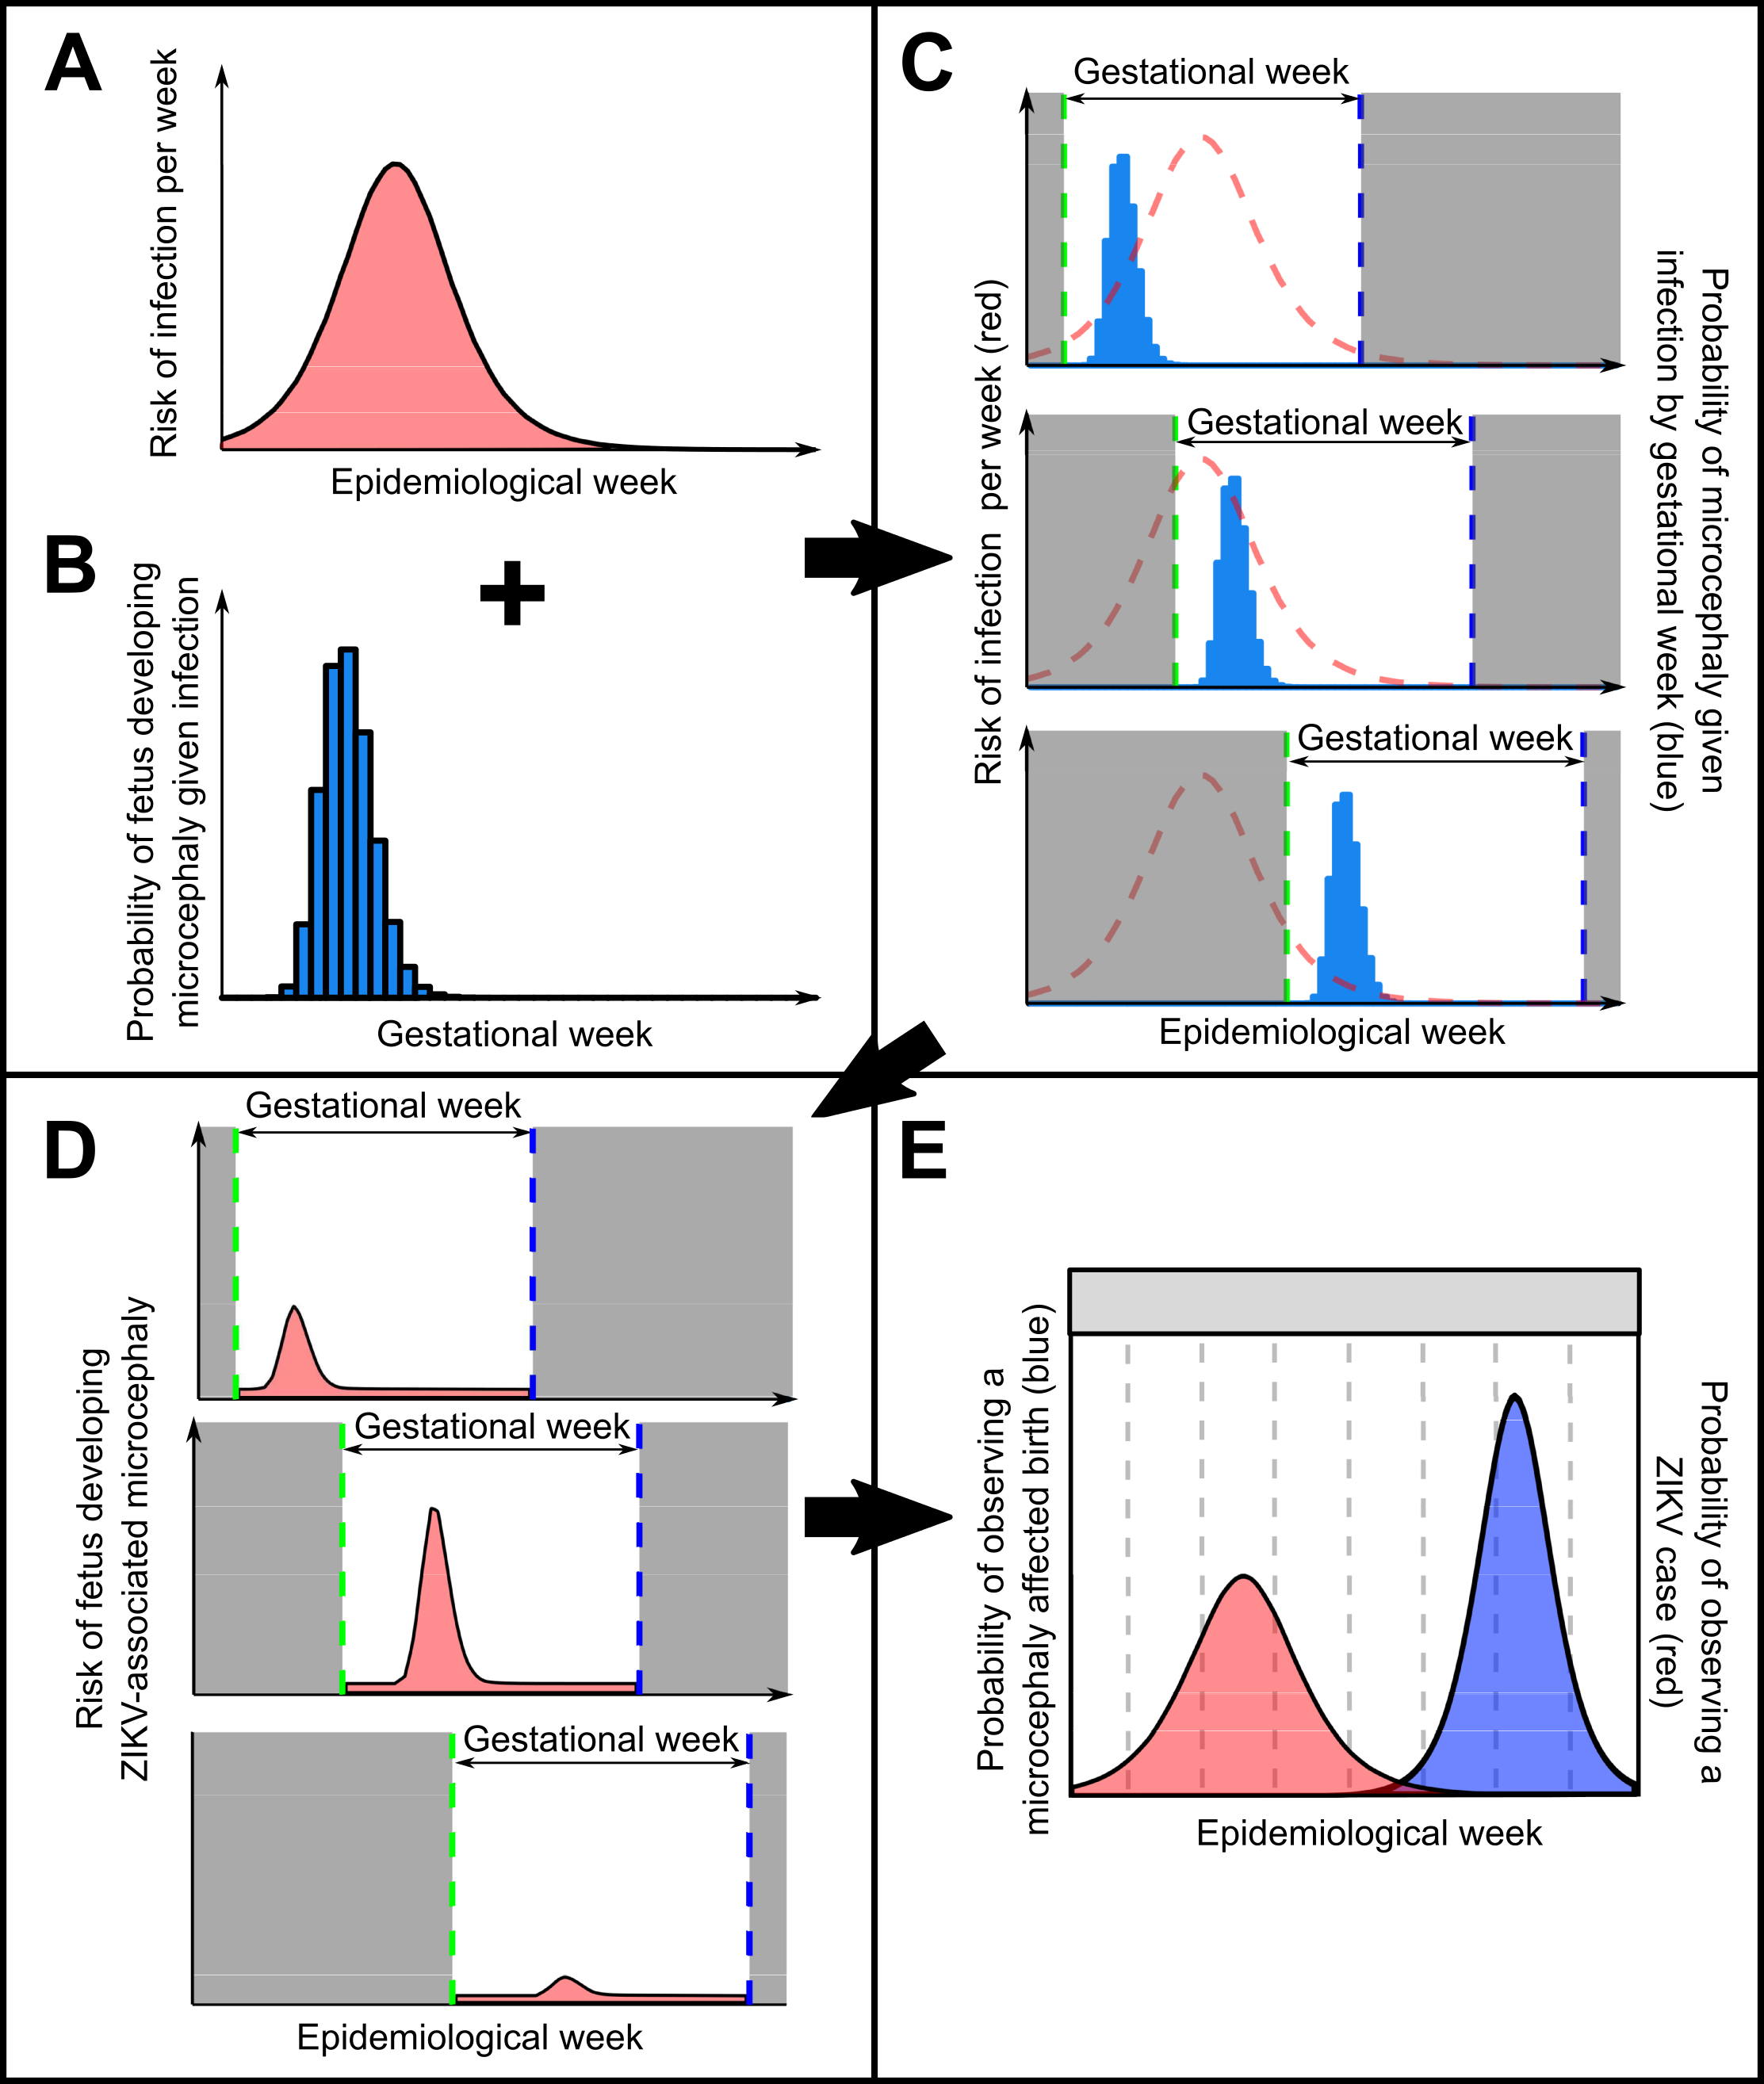
\includegraphics[width=5.20833in]{figures/Fig1.png}
\caption{\textbf{Graphical representation of the SEIR model.} Mosquito
vector population is shown in green, with new mosquitoes entering the
susceptible class (S\textsubscript{M}) and progressing through to the
infected state. The human population is shown in blue, with new humans
entering as susceptible (S\textsubscript{H}). Humans become infected at
a rate of \(\lambda_H\), and become infectious at a rate of
\(\alpha_H\). Humans then recover at a rate of \(\gamma_H\). Note that
the force of infection on humans comes from mosquitoes only, as
represented by the orange arrows. All compartments experience a death
rate of 1/L, where \(L\) is the lifespan in days.}
\end{figure}

Through calculation of the force of infection over time, we estimated a
per capita risk of infection per unit time. The force of infection for
mosquitoes and humans respectively is given by:

\begin{equation}
\begin{array}{lr}
\lambda_M = bp_{HM}I_H \\
\lambda_H = bp_{MH}I_M
\end{array}
\end{equation}

Where \(b\) is the bite rate per vector; \(p_{MH}\) is the probability
of a bite generating an infection in a human from an infected vector;
\(p_{HM}\) is the probability of a bite generating an infection in a
vector from an infected human; and \(I_H\)/\(I_M\) is the number of
infected humans/mosquitoes.

Using this force of infection term, we defined the probability of an
individual not becoming infected at a given time, \(t\), as:{[}2{]}

\begin{equation}
 f(t) = \exp(-\lambda_H(t) \delta t)
\end{equation}

Where \(f(t)\) is the probability of remaining susceptible between \(t\)
and \(t + \delta t\). Here, we used \(\delta t = 1\) day (approximately
\(1/20\)th of the assumed generation time) to approximate the
probability of remaining susceptible within a small, discrete period of
time. We validated this choice of time step by testing values for
\(\delta t\) between 0.1 and 2, which did not affect the model results.
Smaller values of \(\delta t\) were not used for computational reasons.
We calculated the probability of remaining susceptible from \(t_0\) up
to a given time, \(t\), as:

\begin{equation}
F(t) = \prod_{i=t_0}^t f(i)
\end{equation}

Finally, the probability of becoming infected at a given period of time,
\(t\), was defined as:

\begin{equation}
P_{I}(t) = F(t)(1-f(t))
\end{equation}

Where \(P_I(t)\) is the probability of becoming infected between \(t\)
and \(t + \delta t\), given by the probability of remaining susceptible
up to that point multiplied by the probability of not remaining
susceptible during the small time period defined by \(\delta t\). Note
that \(F(t)\) refers to the period of time up to \(t\), whereas \(f(t)\)
refers to the period of time between \(t\) and \(t + \delta t\). Note
also that \(t\) is treated as a discrete unit here to approximate the
theoretical relationship between time-varying force of infection and
infection risk.{[}2{]}

The basic reproductive number, \(R_0\), was defined as the number of new
human infections generated by the introduction of a single infected
human into a naive human and mosquito population given by:{[}3{]}

\begin{equation}
R_0 = \frac{b^2p_{HM}p_{MH}N_M}{\mu_M(\sigma_M + \mu_M)(\gamma_H + \mu_H)N_H}
\end{equation}

Where \(N_M\) is the total number of mosquitoes; \(N_H\) is the total
number of humans; \(\mu_M\) is the birth/death rate of mosquitoes;
\(\sigma_M\) is the rate at which mosquitoes leave the exposed class;
\(\sigma_H\) is the rate at which humans leave the exposed class;
\(\gamma_H\) is the rate at which humans leave the infected class; and
\(\mu_H\) is the birth/death rate of the human population. Critical
values for \(R_0\) were used to validate model implementation (values
at, just above and below 1). We also validated the use of \(R_0\) within
the standard final-size equation to calculate the proportion of exposed
individuals at the end of a single epidemic peak, which allowed to the
calculation the final attack rate based on \(R_0\).{[}2{]}

All biological parameters related to transmission properties and course
of infection were assumed to be the same for all locations, whereas
parameters relating to life expectancy, population size, vector density
(the free component of \(R_0\)) and seeding time (\(t_0\)) were
estimated and assumed to be location specific. Human life expectancy and
population size were assumed to be known and fixed based on official
statistics.{[}4{]} We assumed a fixed mosquito lifespan of 5 days, and
fixed other model parameters such that the generation time of ZIKV was
assumed to be \textasciitilde{}20 days in line with previously published
analyses on Zika transmission.{[}8{]} A sensitivity analysis was run
where mosquito lifespan was fixed at 7 days, but this did not have a
significant impact on the inferred microcephaly risk profile, although
we note that \(R_0\) estimates are conditional on the assumed generation
time. A table summarising the chosen model parameters and their sources
can be found in Table S2.

\subsection{Microcephaly risk model}\label{microcephaly-risk-model}

The second component of the model described the risk of a fetus
developing microcephaly given that the mother was infected in a
particular week during pregnancy. Fitting this risk profile as a curve
rather than a set of per-trimester risk estimates captures more
information regarding the width and shape of the
gestational-time-varying risk profile at the resolution of weeks or days
rather than per trimester. We used a scaled gamma distribution to
characterise the shape and scale of this curve with only 3 free
parameters - the shape, scale, and an additional scaling constant to
increase the magnitude of the curve. This additional scaling constant
was required as the sum under the risk profile did not need to sum to 1
as in the unmodified gamma distribution. The probability of developing
microcephaly given infection was described as:

\begin{equation}
P'_m(x) = \frac{c}{\Gamma(x)\theta^k }x^{k-1}e^{-\frac{x}{\theta}}
\end{equation}

Where \(P'_m(x)\) is the probability of developing microcephaly given
infection in gestational week \(x\) (0 to 39, where 0 is the first week
of pregnancy); \(c\) is an additional scaling constant; \(\theta\) is
the gamma scale parameter; and \(k\) is the gamma shape parameter. The
gamma distribution was chosen due to the flexible shape of the curve
defined by a small number of parameters. Note that \(\theta\) and \(k\)
can be trivially manipulated to give the mean, mode and variance of the
gamma curve. The gamma distribution, \(\Gamma\) was defined as:

\begin{equation}
\Gamma ( x ) = \int\limits_0^\infty {t^{x - 1} } e^{ - t} dt
\end{equation}

\subsection{Combined model}\label{combined-model}

Based on the transmission model and microcephaly risk model, the
expected proportion of microcephaly affected births (Figure 1E) was
calculated by multiplying these two components together. The probability
of ZIKV-associated microcephaly affected birth at time, \(t\), was
therefore given by:

\begin{equation}
 P_m(t) = \sum^t_{i=t-40} P_I(i)P'_m(i - t + 40)
\end{equation}

Where \(P_m(t)\) is the per live birth probability of a ZIKV-associated
microcephaly birth at time \(t\), \(P_I(i)\) is the probability of an
individual becoming infected at time \(i\) (and not before), and
\(P'_m(i - t + 40)\) is the probability of fetus developing microcephaly
given ZIKV infection at gestational week \(i - t + 40\). Essentially,
the probability of a live birth being affected by ZIKV-associated
microcephaly is the sum of all of the opportunities that the mother
could have been infected and the fetus subsequently developed
microcephaly in each of the 40 weeks of pregnancy preceding the birth.

Including a baseline microcephaly rate (ie. not associated with ZIKV)
gives the probability of observing any microcephaly case at time \(t\)
as:

\begin{equation}
 P_{micro}(t) =\phi_{m,i}(1 - (1-P_m(t))(1-P_b))
\end{equation}

Where \(P_b\) is the baseline per birth microcephaly incidence rate and
\(\phi_{m,i}\) is the proportion of true cases that were reported in
location \(i\) (less than one indicates underreporting, greater than one
indicates overreporting). Multiplying this proportion by the total
number of live births at time \(t\), \(B(t)\), gives the expected number
of observed microcephaly-affected births at time \(t\).

\section{Data}\label{data}

\subsection{Microcephaly and ZIKV incidence
data}\label{microcephaly-and-zikv-incidence-data}

We searched the literature and Brazilian state health authority websites
for reports of suspected ZIKV incidence and microcephaly cases in 2015
and early 2016, as described in the main text. To recap: we searched
\href{www.paho.org}{www.paho.org}, \href{www.who.int}{www.who.int},
Brazilian state-level ministry of health websites (eg.
\href{www.suvisa.ba.gov.br}{www.suvisa.ba.gov.br}), and PubMed for the
terms ``zika'' and ``microcephaly''.

ZIKV and microcephaly incidence data from 2015 were available from
publications and epidemiological reports for the states of Pernambuco,
Rio Grande do Norte and Bahia (at state level and for the city of
Salvador), though no useable data sets from 2015 were found for any
other state. Monthly microcephaly incidence and births by state was also
found online from the SINASC/CGIAE/SVS/MS system as reported
previously.{[}9{]} An additional source of ZIKV incidence for all
Brazilian states was also obtained from a publication in 2016;{[}11{]}
however, the timing of the epidemic peak in these data suggested that
incidence peaked in July 2015, contrasting with state-level reports
which suggested an earlier peak. We also considered preliminary and
later confirmed data ZIKV and microcephaly incidence published from the
Brazilian ministry of health, which suggested a later ZIKV infection
peak time compared to early state-level reports.{[}12{]} Microcephaly
and ZIKV incidence data were obtained for Colombia at the national
level.{[}14{]} Finally, we found confirmed microcephaly case data for
some locations (Rio Grande do Norte, Pernambuco, Northeast Brazil
aggregated) and also confirmed ZIKV infection incidence for Colombia.
Confirmed case reports were available for Colombia from weekly
epidemiological bulletins; however, these did not include the date of
report of confirmed cases, and we were therefore unable to extract
incidence from reported cumulative cases.{[}16{]}

A summary of data included in the analyses can be found in Table S1.
Some data sources were only available in graphical form, and these
numbers were therefore extracted using a web digitizer
(\href{https://automeris.io/WebPlotDigitizer/}{https://automeris.io/WebPlotDigitizer/}).
The results presented in the main text used:

\begin{enumerate}
\item Aggregated weekly confirmed microcephaly and notified ZIKV infection in pregnant women incidence data from Northeast Brazil; 
\item Weekly confirmed/notified ZIKV infection and notified microcephaly incidence data from Colombia; 
\item State-reported weekly notified microcephaly and ZIKV incidence from Bahia, Brazil; 
\item State-reported confirmed weekly microcephaly incidence from Pernambuco, Brazil; 
\item State-reported monthly confirmed/notified microcephaly and notified ZIKV incidence from Rio Grande do Norte; 
\item Reported acute exanthematous illness (AEI) and notified microcephaly incidence from the city of Salvador, Bahia, Brazil (see below). 
\end{enumerate}

Model fitting using other data sources for the same locations, as well
as fitting a single microcephaly risk profile to data from multiple
locations simultaneously, was carried out but results are not presented
here. Different data sources for the same location produced
qualitatively similar risk profile estimates in terms of the window and
timing of risk.

Numbers of live births were obtained for Brazil from the
SINASC/CGIAE/SVS/MS system.{[}9{]} For Colombia, live births were
obtained from a publication of microcephaly and ZIKV incidence in
Colombia and ratified against country wide statistics.{[}15{]} Where
reporting of live births was incomplete, we estimated the number of live
births by averaging the number of births in the previous two years for
the same dates. Where birth data was only available at a lower time
resolution than reported incidence data, we assumed that the total
number of births for that year were uniformly distributed across each
day.

Extraction of incidence data from {[}13{]} was slightly more involved,
as exact microcephaly case numbers were not provided. However, we were
able to estimate the case count data given the methodology in this
publication. {[}13{]} reported confirmed microcephaly incidence per
10,000 births and notified ZIKV infection incidence per 10,000 pregnant
women, as well as the total number of microcephaly cases and monthly
number of infected pregnant women. We could therefore infer the number
of monthly births as follows:

\begin{equation}
 \begin{array}{lr}
 \text{pregnant women(t)} = (\text{births(t)}*9) + (\text{births}*0.2)*1.5 \\
\text{pregnant women(t)} = \text{births(t)}*9.3 \\
 \text{births(t)} = \text{pregnant women(t)}/9.3
\end{array}
\end{equation}

Where \(\text{pregnant women(t)}\) is the number of pregnant women in
month \(t\) (which is known) and \(\text{births(t)}\) is the number of
births in month \(t\). We then infer the number of microcephaly cases
per month as:

\begin{equation}
\text{microcephaly cases(t)} = \text{births(t)}*\text{microceph incidence(t)}
\end{equation}

Where \(\text{microcephaly cases(t)}\) is the number of microcephaly
cases reported in month \(t\) and \(\text{microceph incidence(t)}\) is
the per birth incidence of microcephaly in month \(t\).

Note that we use the total population size for Northeast Brazil as the
denominator for per capita incidence, as the reporting rate parameter
(described below) accounts for the fact that infected pregnant women
only represent a fraction of the true infected population.

All data are available to download in human readable form in the
accompanying R package
\href{https://github.com/jameshay218/zikaInfer/tree/master/RawData/}{here}.
The files
\href{https://github.com/jameshay218/zikaInfer/tree/master/RawData/data_sources.csv}{\texttt{data\_sources.csv}}
and
\href{https://github.com/jameshay218/zikaInfer/tree/master/RawData/data_key.csv}{\texttt{data\_key.csv}}
describe the sources of these data and the column names respectively.
Note that \texttt{startDay} and \texttt{endDay} refer to the first and
last day that the reporting period covers; \texttt{buckets} refers to
the number of days that that reporting window covers; and all dates were
converted to integers (where 1 day = 1), and 01/01/2013 was taken as day
0.

\textbf{Table S1: Summary of datasets included in the analysis.}
\emph{For each location, the type of incidence data, the time resolution
of reports, whether or not data were extracted using a digitiser and the
data source are provided. Sources refer to references in the main text.}
\tiny

\begin{longtable}[]{@{}lllllll@{}}
\toprule
\begin{minipage}[b]{0.03\columnwidth}\raggedright\strut
Country\strut
\end{minipage} & \begin{minipage}[b]{0.37\columnwidth}\raggedright\strut
Location\strut
\end{minipage} & \begin{minipage}[b]{0.08\columnwidth}\raggedright\strut
Incidence type\strut
\end{minipage} & \begin{minipage}[b]{0.17\columnwidth}\raggedright\strut
Reported or Confirmed?\strut
\end{minipage} & \begin{minipage}[b]{0.04\columnwidth}\raggedright\strut
Resolution\strut
\end{minipage} & \begin{minipage}[b]{0.04\columnwidth}\raggedright\strut
Digitised?\strut
\end{minipage} & \begin{minipage}[b]{0.08\columnwidth}\raggedright\strut
Source\strut
\end{minipage}\tabularnewline
\midrule
\endhead
\begin{minipage}[t]{0.03\columnwidth}\raggedright\strut
Brazil\strut
\end{minipage} & \begin{minipage}[t]{0.37\columnwidth}\raggedright\strut
Northeast states (Alagoas, Bahia, Ceará, Maranhão, Paraíba, Pernambuco,
Piauí, Rio Grande do Norte and Sergipe)\strut
\end{minipage} & \begin{minipage}[t]{0.08\columnwidth}\raggedright\strut
Microcephaly and ZIKV\strut
\end{minipage} & \begin{minipage}[t]{0.17\columnwidth}\raggedright\strut
Microcephaly confirmed; ZIKV reported\strut
\end{minipage} & \begin{minipage}[t]{0.04\columnwidth}\raggedright\strut
Weekly\strut
\end{minipage} & \begin{minipage}[t]{0.04\columnwidth}\raggedright\strut
No\strut
\end{minipage} & \begin{minipage}[t]{0.08\columnwidth}\raggedright\strut
{[}12{]}\strut
\end{minipage}\tabularnewline
\begin{minipage}[t]{0.03\columnwidth}\raggedright\strut
Brazil\strut
\end{minipage} & \begin{minipage}[t]{0.37\columnwidth}\raggedright\strut
Northeast states (Alagoas, Bahia, Ceará, Maranhão, Paraíba, Pernambuco,
Piauí, Rio Grande do Norte and Sergipe)\strut
\end{minipage} & \begin{minipage}[t]{0.08\columnwidth}\raggedright\strut
Microcephaly and ZIKV\strut
\end{minipage} & \begin{minipage}[t]{0.17\columnwidth}\raggedright\strut
Microcephaly confirmed \& predicted; ZIKV reported\strut
\end{minipage} & \begin{minipage}[t]{0.04\columnwidth}\raggedright\strut
Weekly\strut
\end{minipage} & \begin{minipage}[t]{0.04\columnwidth}\raggedright\strut
Yes\strut
\end{minipage} & \begin{minipage}[t]{0.08\columnwidth}\raggedright\strut
{[}13{]}\strut
\end{minipage}\tabularnewline
\begin{minipage}[t]{0.03\columnwidth}\raggedright\strut
Colombia\strut
\end{minipage} & \begin{minipage}[t]{0.37\columnwidth}\raggedright\strut
Country-wide\strut
\end{minipage} & \begin{minipage}[t]{0.08\columnwidth}\raggedright\strut
Microcephaly\strut
\end{minipage} & \begin{minipage}[t]{0.17\columnwidth}\raggedright\strut
Reported\strut
\end{minipage} & \begin{minipage}[t]{0.04\columnwidth}\raggedright\strut
Weekly\strut
\end{minipage} & \begin{minipage}[t]{0.04\columnwidth}\raggedright\strut
Yes\strut
\end{minipage} & \begin{minipage}[t]{0.08\columnwidth}\raggedright\strut
{[}14{]}\strut
\end{minipage}\tabularnewline
\begin{minipage}[t]{0.03\columnwidth}\raggedright\strut
Colombia\strut
\end{minipage} & \begin{minipage}[t]{0.37\columnwidth}\raggedright\strut
Country-wide\strut
\end{minipage} & \begin{minipage}[t]{0.08\columnwidth}\raggedright\strut
ZIKV\strut
\end{minipage} & \begin{minipage}[t]{0.17\columnwidth}\raggedright\strut
Reported\strut
\end{minipage} & \begin{minipage}[t]{0.04\columnwidth}\raggedright\strut
Weekly\strut
\end{minipage} & \begin{minipage}[t]{0.04\columnwidth}\raggedright\strut
Yes\strut
\end{minipage} & \begin{minipage}[t]{0.08\columnwidth}\raggedright\strut
{[}14{]}\strut
\end{minipage}\tabularnewline
\begin{minipage}[t]{0.03\columnwidth}\raggedright\strut
Colombia\strut
\end{minipage} & \begin{minipage}[t]{0.37\columnwidth}\raggedright\strut
Country-wide\strut
\end{minipage} & \begin{minipage}[t]{0.08\columnwidth}\raggedright\strut
ZIKV\strut
\end{minipage} & \begin{minipage}[t]{0.17\columnwidth}\raggedright\strut
Confirmed\strut
\end{minipage} & \begin{minipage}[t]{0.04\columnwidth}\raggedright\strut
Weekly\strut
\end{minipage} & \begin{minipage}[t]{0.04\columnwidth}\raggedright\strut
Yes\strut
\end{minipage} & \begin{minipage}[t]{0.08\columnwidth}\raggedright\strut
{[}14{]}\strut
\end{minipage}\tabularnewline
\begin{minipage}[t]{0.03\columnwidth}\raggedright\strut
Colombia\strut
\end{minipage} & \begin{minipage}[t]{0.37\columnwidth}\raggedright\strut
Country-wide\strut
\end{minipage} & \begin{minipage}[t]{0.08\columnwidth}\raggedright\strut
Microcephaly\strut
\end{minipage} & \begin{minipage}[t]{0.17\columnwidth}\raggedright\strut
Reported\strut
\end{minipage} & \begin{minipage}[t]{0.04\columnwidth}\raggedright\strut
Monthly\strut
\end{minipage} & \begin{minipage}[t]{0.04\columnwidth}\raggedright\strut
No\strut
\end{minipage} & \begin{minipage}[t]{0.08\columnwidth}\raggedright\strut
{[}15{]}\strut
\end{minipage}\tabularnewline
\begin{minipage}[t]{0.03\columnwidth}\raggedright\strut
Colombia\strut
\end{minipage} & \begin{minipage}[t]{0.37\columnwidth}\raggedright\strut
Country-wide\strut
\end{minipage} & \begin{minipage}[t]{0.08\columnwidth}\raggedright\strut
Microcephaly\strut
\end{minipage} & \begin{minipage}[t]{0.17\columnwidth}\raggedright\strut
Reported\strut
\end{minipage} & \begin{minipage}[t]{0.04\columnwidth}\raggedright\strut
Weekly\strut
\end{minipage} & \begin{minipage}[t]{0.04\columnwidth}\raggedright\strut
No\strut
\end{minipage} & \begin{minipage}[t]{0.08\columnwidth}\raggedright\strut
{[}16{]}\strut
\end{minipage}\tabularnewline
\begin{minipage}[t]{0.03\columnwidth}\raggedright\strut
Colombia\strut
\end{minipage} & \begin{minipage}[t]{0.37\columnwidth}\raggedright\strut
Country-wide\strut
\end{minipage} & \begin{minipage}[t]{0.08\columnwidth}\raggedright\strut
Microcephaly\strut
\end{minipage} & \begin{minipage}[t]{0.17\columnwidth}\raggedright\strut
Confirmed\strut
\end{minipage} & \begin{minipage}[t]{0.04\columnwidth}\raggedright\strut
Weekly\strut
\end{minipage} & \begin{minipage}[t]{0.04\columnwidth}\raggedright\strut
No\strut
\end{minipage} & \begin{minipage}[t]{0.08\columnwidth}\raggedright\strut
{[}16{]}\strut
\end{minipage}\tabularnewline
\begin{minipage}[t]{0.03\columnwidth}\raggedright\strut
Brazil\strut
\end{minipage} & \begin{minipage}[t]{0.37\columnwidth}\raggedright\strut
Bahia\strut
\end{minipage} & \begin{minipage}[t]{0.08\columnwidth}\raggedright\strut
Microcephaly\strut
\end{minipage} & \begin{minipage}[t]{0.17\columnwidth}\raggedright\strut
Reported\strut
\end{minipage} & \begin{minipage}[t]{0.04\columnwidth}\raggedright\strut
Weekly\strut
\end{minipage} & \begin{minipage}[t]{0.04\columnwidth}\raggedright\strut
Yes\strut
\end{minipage} & \begin{minipage}[t]{0.08\columnwidth}\raggedright\strut
{[}17{]}\strut
\end{minipage}\tabularnewline
\begin{minipage}[t]{0.03\columnwidth}\raggedright\strut
Brazil\strut
\end{minipage} & \begin{minipage}[t]{0.37\columnwidth}\raggedright\strut
Bahia\strut
\end{minipage} & \begin{minipage}[t]{0.08\columnwidth}\raggedright\strut
Microcephaly\strut
\end{minipage} & \begin{minipage}[t]{0.17\columnwidth}\raggedright\strut
Reported\strut
\end{minipage} & \begin{minipage}[t]{0.04\columnwidth}\raggedright\strut
Monthly\strut
\end{minipage} & \begin{minipage}[t]{0.04\columnwidth}\raggedright\strut
No\strut
\end{minipage} & \begin{minipage}[t]{0.08\columnwidth}\raggedright\strut
{[}10{]}\strut
\end{minipage}\tabularnewline
\begin{minipage}[t]{0.03\columnwidth}\raggedright\strut
Brazil\strut
\end{minipage} & \begin{minipage}[t]{0.37\columnwidth}\raggedright\strut
Bahia\strut
\end{minipage} & \begin{minipage}[t]{0.08\columnwidth}\raggedright\strut
ZIKV\strut
\end{minipage} & \begin{minipage}[t]{0.17\columnwidth}\raggedright\strut
Reported\strut
\end{minipage} & \begin{minipage}[t]{0.04\columnwidth}\raggedright\strut
Weekly\strut
\end{minipage} & \begin{minipage}[t]{0.04\columnwidth}\raggedright\strut
Yes\strut
\end{minipage} & \begin{minipage}[t]{0.08\columnwidth}\raggedright\strut
{[}18{]}\strut
\end{minipage}\tabularnewline
\begin{minipage}[t]{0.03\columnwidth}\raggedright\strut
Brazil\strut
\end{minipage} & \begin{minipage}[t]{0.37\columnwidth}\raggedright\strut
Rio Grande do Norte\strut
\end{minipage} & \begin{minipage}[t]{0.08\columnwidth}\raggedright\strut
Microcephaly\strut
\end{minipage} & \begin{minipage}[t]{0.17\columnwidth}\raggedright\strut
Reported\strut
\end{minipage} & \begin{minipage}[t]{0.04\columnwidth}\raggedright\strut
Monthly\strut
\end{minipage} & \begin{minipage}[t]{0.04\columnwidth}\raggedright\strut
No\strut
\end{minipage} & \begin{minipage}[t]{0.08\columnwidth}\raggedright\strut
{[}19{]}\strut
\end{minipage}\tabularnewline
\begin{minipage}[t]{0.03\columnwidth}\raggedright\strut
Brazil\strut
\end{minipage} & \begin{minipage}[t]{0.37\columnwidth}\raggedright\strut
Rio Grande do Norte\strut
\end{minipage} & \begin{minipage}[t]{0.08\columnwidth}\raggedright\strut
Microcephaly\strut
\end{minipage} & \begin{minipage}[t]{0.17\columnwidth}\raggedright\strut
Confirmed\strut
\end{minipage} & \begin{minipage}[t]{0.04\columnwidth}\raggedright\strut
Monthly\strut
\end{minipage} & \begin{minipage}[t]{0.04\columnwidth}\raggedright\strut
Yes\strut
\end{minipage} & \begin{minipage}[t]{0.08\columnwidth}\raggedright\strut
{[}19{]}\strut
\end{minipage}\tabularnewline
\begin{minipage}[t]{0.03\columnwidth}\raggedright\strut
Brazil\strut
\end{minipage} & \begin{minipage}[t]{0.37\columnwidth}\raggedright\strut
Rio Grande do Norte\strut
\end{minipage} & \begin{minipage}[t]{0.08\columnwidth}\raggedright\strut
Microcephaly\strut
\end{minipage} & \begin{minipage}[t]{0.17\columnwidth}\raggedright\strut
Reported\strut
\end{minipage} & \begin{minipage}[t]{0.04\columnwidth}\raggedright\strut
Monthly\strut
\end{minipage} & \begin{minipage}[t]{0.04\columnwidth}\raggedright\strut
No\strut
\end{minipage} & \begin{minipage}[t]{0.08\columnwidth}\raggedright\strut
{[}10{]}\strut
\end{minipage}\tabularnewline
\begin{minipage}[t]{0.03\columnwidth}\raggedright\strut
Brazil\strut
\end{minipage} & \begin{minipage}[t]{0.37\columnwidth}\raggedright\strut
Rio Grande do Norte\strut
\end{minipage} & \begin{minipage}[t]{0.08\columnwidth}\raggedright\strut
ZIKV\strut
\end{minipage} & \begin{minipage}[t]{0.17\columnwidth}\raggedright\strut
Reported\strut
\end{minipage} & \begin{minipage}[t]{0.04\columnwidth}\raggedright\strut
Weekly\strut
\end{minipage} & \begin{minipage}[t]{0.04\columnwidth}\raggedright\strut
Yes\strut
\end{minipage} & \begin{minipage}[t]{0.08\columnwidth}\raggedright\strut
{[}20{]}\strut
\end{minipage}\tabularnewline
\begin{minipage}[t]{0.03\columnwidth}\raggedright\strut
Brazil\strut
\end{minipage} & \begin{minipage}[t]{0.37\columnwidth}\raggedright\strut
Pernambuco\strut
\end{minipage} & \begin{minipage}[t]{0.08\columnwidth}\raggedright\strut
Microcephaly\strut
\end{minipage} & \begin{minipage}[t]{0.17\columnwidth}\raggedright\strut
Confirmed \& Reported\strut
\end{minipage} & \begin{minipage}[t]{0.04\columnwidth}\raggedright\strut
Weekly\strut
\end{minipage} & \begin{minipage}[t]{0.04\columnwidth}\raggedright\strut
Yes\strut
\end{minipage} & \begin{minipage}[t]{0.08\columnwidth}\raggedright\strut
{[}21{]}\strut
\end{minipage}\tabularnewline
\begin{minipage}[t]{0.03\columnwidth}\raggedright\strut
Brazil\strut
\end{minipage} & \begin{minipage}[t]{0.37\columnwidth}\raggedright\strut
Pernambuco\strut
\end{minipage} & \begin{minipage}[t]{0.08\columnwidth}\raggedright\strut
ZIKV\strut
\end{minipage} & \begin{minipage}[t]{0.17\columnwidth}\raggedright\strut
Reported\strut
\end{minipage} & \begin{minipage}[t]{0.04\columnwidth}\raggedright\strut
Weekly\strut
\end{minipage} & \begin{minipage}[t]{0.04\columnwidth}\raggedright\strut
Yes\strut
\end{minipage} & \begin{minipage}[t]{0.08\columnwidth}\raggedright\strut
{[}22{]}\strut
\end{minipage}\tabularnewline
\begin{minipage}[t]{0.03\columnwidth}\raggedright\strut
Brazil\strut
\end{minipage} & \begin{minipage}[t]{0.37\columnwidth}\raggedright\strut
Pernambuco\strut
\end{minipage} & \begin{minipage}[t]{0.08\columnwidth}\raggedright\strut
Microcephaly\strut
\end{minipage} & \begin{minipage}[t]{0.17\columnwidth}\raggedright\strut
Reported\strut
\end{minipage} & \begin{minipage}[t]{0.04\columnwidth}\raggedright\strut
Monthly\strut
\end{minipage} & \begin{minipage}[t]{0.04\columnwidth}\raggedright\strut
No\strut
\end{minipage} & \begin{minipage}[t]{0.08\columnwidth}\raggedright\strut
{[}10{]}\strut
\end{minipage}\tabularnewline
\begin{minipage}[t]{0.03\columnwidth}\raggedright\strut
Brazil\strut
\end{minipage} & \begin{minipage}[t]{0.37\columnwidth}\raggedright\strut
Salvador, Bahia\strut
\end{minipage} & \begin{minipage}[t]{0.08\columnwidth}\raggedright\strut
ZIKV\strut
\end{minipage} & \begin{minipage}[t]{0.17\columnwidth}\raggedright\strut
Reported\strut
\end{minipage} & \begin{minipage}[t]{0.04\columnwidth}\raggedright\strut
Weekly\strut
\end{minipage} & \begin{minipage}[t]{0.04\columnwidth}\raggedright\strut
No\strut
\end{minipage} & \begin{minipage}[t]{0.08\columnwidth}\raggedright\strut
{[}23{]}\strut
\end{minipage}\tabularnewline
\begin{minipage}[t]{0.03\columnwidth}\raggedright\strut
Brazil\strut
\end{minipage} & \begin{minipage}[t]{0.37\columnwidth}\raggedright\strut
Salvador, Bahia\strut
\end{minipage} & \begin{minipage}[t]{0.08\columnwidth}\raggedright\strut
Microcephaly\strut
\end{minipage} & \begin{minipage}[t]{0.17\columnwidth}\raggedright\strut
Reported\strut
\end{minipage} & \begin{minipage}[t]{0.04\columnwidth}\raggedright\strut
Weekly\strut
\end{minipage} & \begin{minipage}[t]{0.04\columnwidth}\raggedright\strut
No\strut
\end{minipage} & \begin{minipage}[t]{0.08\columnwidth}\raggedright\strut
{[}23{]}\strut
\end{minipage}\tabularnewline
\bottomrule
\end{longtable}

\normalsize

\subsection{Model parameters}\label{model-parameters}

Model parameters related to ZIKV transmission were obtained from the
literature as described in Table S2. Parameters were predominately
chosen based on a previously published transmission model, with point
values chosen to give a generation time of approximately 20 days.{[}8{]}
Values used were as described in Table S6 of {[}8{]}, with the intrinsic
latency period here taken as the intrinsic incubation period described
in {[}8{]} less 1.5 days to reflect the assumption that infectiousness
starts 1.5 days before symptom onset. Given a fixed generation time, the
shape of the SEIR model predicted incidence curve was allowed to vary
depending on the value of \(R_0\). As \(R_0\) is comprised of multiple
correlated parameters, all components of \(R_0\) other than the vector
density per human were fixed. Vital statistics (human life expectancy
and population size) for particular locations are described in Table S3.

\textbf{Table S2. Summary of model parameters, sources and assumed
parameter ranges.} \emph{Parameter symbols are as described in the text.
The component column refers to which part of the model or which part of
the analysis that parameter relates. Values shown are the fixed point
values used in the analysis or estimated. Where specified, lower and
upper bounds refer to prior ranges imposed during the MCMC fitting.
Sources refer to references in the main text.} \tiny

\begin{longtable}[]{@{}llllllll@{}}
\toprule
\begin{minipage}[b]{0.04\columnwidth}\raggedright\strut
Parameter\strut
\end{minipage} & \begin{minipage}[b]{0.17\columnwidth}\raggedright\strut
Description\strut
\end{minipage} & \begin{minipage}[b]{0.05\columnwidth}\raggedright\strut
Component\strut
\end{minipage} & \begin{minipage}[b]{0.05\columnwidth}\raggedright\strut
Value\strut
\end{minipage} & \begin{minipage}[b]{0.04\columnwidth}\raggedright\strut
Lower Bound\strut
\end{minipage} & \begin{minipage}[b]{0.04\columnwidth}\raggedright\strut
Upper Bound\strut
\end{minipage} & \begin{minipage}[b]{0.14\columnwidth}\raggedright\strut
Source\strut
\end{minipage} & \begin{minipage}[b]{0.26\columnwidth}\raggedright\strut
Notes\strut
\end{minipage}\tabularnewline
\midrule
\endhead
\begin{minipage}[t]{0.04\columnwidth}\raggedright\strut
\(1/\mu_M\)\strut
\end{minipage} & \begin{minipage}[t]{0.17\columnwidth}\raggedright\strut
Lifespan of mosquitoes\strut
\end{minipage} & \begin{minipage}[t]{0.05\columnwidth}\raggedright\strut
SEIR\strut
\end{minipage} & \begin{minipage}[t]{0.05\columnwidth}\raggedright\strut
5 days\strut
\end{minipage} & \begin{minipage}[t]{0.04\columnwidth}\raggedright\strut
N/A\strut
\end{minipage} & \begin{minipage}[t]{0.04\columnwidth}\raggedright\strut
N/A\strut
\end{minipage} & \begin{minipage}[t]{0.14\columnwidth}\raggedright\strut
{[}8{]}, {[}24{]}\strut
\end{minipage} & \begin{minipage}[t]{0.26\columnwidth}\raggedright\strut
\strut
\end{minipage}\tabularnewline
\begin{minipage}[t]{0.04\columnwidth}\raggedright\strut
\(\sigma_H\)\strut
\end{minipage} & \begin{minipage}[t]{0.17\columnwidth}\raggedright\strut
Intrinsic latency period\strut
\end{minipage} & \begin{minipage}[t]{0.05\columnwidth}\raggedright\strut
SEIR\strut
\end{minipage} & \begin{minipage}[t]{0.05\columnwidth}\raggedright\strut
4 days\strut
\end{minipage} & \begin{minipage}[t]{0.04\columnwidth}\raggedright\strut
N/A\strut
\end{minipage} & \begin{minipage}[t]{0.04\columnwidth}\raggedright\strut
N/A\strut
\end{minipage} & \begin{minipage}[t]{0.14\columnwidth}\raggedright\strut
{[}25{]}, {[}8{]}\strut
\end{minipage} & \begin{minipage}[t]{0.26\columnwidth}\raggedright\strut
\strut
\end{minipage}\tabularnewline
\begin{minipage}[t]{0.04\columnwidth}\raggedright\strut
\(\sigma_M\)\strut
\end{minipage} & \begin{minipage}[t]{0.17\columnwidth}\raggedright\strut
Extrinsic latency period\strut
\end{minipage} & \begin{minipage}[t]{0.05\columnwidth}\raggedright\strut
SEIR\strut
\end{minipage} & \begin{minipage}[t]{0.05\columnwidth}\raggedright\strut
8.4 days\strut
\end{minipage} & \begin{minipage}[t]{0.04\columnwidth}\raggedright\strut
N/A\strut
\end{minipage} & \begin{minipage}[t]{0.04\columnwidth}\raggedright\strut
N/A\strut
\end{minipage} & \begin{minipage}[t]{0.14\columnwidth}\raggedright\strut
{[}26{]}, {[}8{]}\strut
\end{minipage} & \begin{minipage}[t]{0.26\columnwidth}\raggedright\strut
\strut
\end{minipage}\tabularnewline
\begin{minipage}[t]{0.04\columnwidth}\raggedright\strut
\(\gamma_H\)\strut
\end{minipage} & \begin{minipage}[t]{0.17\columnwidth}\raggedright\strut
Human infectious period\strut
\end{minipage} & \begin{minipage}[t]{0.05\columnwidth}\raggedright\strut
SEIR\strut
\end{minipage} & \begin{minipage}[t]{0.05\columnwidth}\raggedright\strut
6 days\strut
\end{minipage} & \begin{minipage}[t]{0.04\columnwidth}\raggedright\strut
N/A\strut
\end{minipage} & \begin{minipage}[t]{0.04\columnwidth}\raggedright\strut
N/A\strut
\end{minipage} & \begin{minipage}[t]{0.14\columnwidth}\raggedright\strut
{[}26{]}, {[}8{]}\strut
\end{minipage} & \begin{minipage}[t]{0.26\columnwidth}\raggedright\strut
\strut
\end{minipage}\tabularnewline
\begin{minipage}[t]{0.04\columnwidth}\raggedright\strut
\(p_{HM}\)\strut
\end{minipage} & \begin{minipage}[t]{0.17\columnwidth}\raggedright\strut
Probability of transmission from human to mosquito given bite\strut
\end{minipage} & \begin{minipage}[t]{0.05\columnwidth}\raggedright\strut
SEIR\strut
\end{minipage} & \begin{minipage}[t]{0.05\columnwidth}\raggedright\strut
0.5\strut
\end{minipage} & \begin{minipage}[t]{0.04\columnwidth}\raggedright\strut
N/A\strut
\end{minipage} & \begin{minipage}[t]{0.04\columnwidth}\raggedright\strut
N/A\strut
\end{minipage} & \begin{minipage}[t]{0.14\columnwidth}\raggedright\strut
\strut
\end{minipage} & \begin{minipage}[t]{0.26\columnwidth}\raggedright\strut
Arbitrarily fixed - component of R0\strut
\end{minipage}\tabularnewline
\begin{minipage}[t]{0.04\columnwidth}\raggedright\strut
\(p_{MH}\)\strut
\end{minipage} & \begin{minipage}[t]{0.17\columnwidth}\raggedright\strut
Probability of transmission from mosquito to human given bite\strut
\end{minipage} & \begin{minipage}[t]{0.05\columnwidth}\raggedright\strut
SEIR\strut
\end{minipage} & \begin{minipage}[t]{0.05\columnwidth}\raggedright\strut
0.5\strut
\end{minipage} & \begin{minipage}[t]{0.04\columnwidth}\raggedright\strut
N/A\strut
\end{minipage} & \begin{minipage}[t]{0.04\columnwidth}\raggedright\strut
N/A\strut
\end{minipage} & \begin{minipage}[t]{0.14\columnwidth}\raggedright\strut
\strut
\end{minipage} & \begin{minipage}[t]{0.26\columnwidth}\raggedright\strut
Arbitrarily fixed - component of R0\strut
\end{minipage}\tabularnewline
\begin{minipage}[t]{0.04\columnwidth}\raggedright\strut
b\strut
\end{minipage} & \begin{minipage}[t]{0.17\columnwidth}\raggedright\strut
Per vector per day bite rate\strut
\end{minipage} & \begin{minipage}[t]{0.05\columnwidth}\raggedright\strut
SEIR\strut
\end{minipage} & \begin{minipage}[t]{0.05\columnwidth}\raggedright\strut
0.5\strut
\end{minipage} & \begin{minipage}[t]{0.04\columnwidth}\raggedright\strut
N/A\strut
\end{minipage} & \begin{minipage}[t]{0.04\columnwidth}\raggedright\strut
N/A\strut
\end{minipage} & \begin{minipage}[t]{0.14\columnwidth}\raggedright\strut
\strut
\end{minipage} & \begin{minipage}[t]{0.26\columnwidth}\raggedright\strut
Arbitrarily fixed - component of R0\strut
\end{minipage}\tabularnewline
\begin{minipage}[t]{0.04\columnwidth}\raggedright\strut
\(\alpha\)\strut
\end{minipage} & \begin{minipage}[t]{0.17\columnwidth}\raggedright\strut
Microcephaly curve rate parameter (mean/variance)\strut
\end{minipage} & \begin{minipage}[t]{0.05\columnwidth}\raggedright\strut
Gamma risk curve\strut
\end{minipage} & \begin{minipage}[t]{0.05\columnwidth}\raggedright\strut
Estimated\strut
\end{minipage} & \begin{minipage}[t]{0.04\columnwidth}\raggedright\strut
0\strut
\end{minipage} & \begin{minipage}[t]{0.04\columnwidth}\raggedright\strut
10000\strut
\end{minipage} & \begin{minipage}[t]{0.14\columnwidth}\raggedright\strut
\strut
\end{minipage} & \begin{minipage}[t]{0.26\columnwidth}\raggedright\strut
\strut
\end{minipage}\tabularnewline
\begin{minipage}[t]{0.04\columnwidth}\raggedright\strut
\(\beta\)\strut
\end{minipage} & \begin{minipage}[t]{0.17\columnwidth}\raggedright\strut
Microcephaly curve shape parameter (mean*alpha)\strut
\end{minipage} & \begin{minipage}[t]{0.05\columnwidth}\raggedright\strut
Gamma risk curve\strut
\end{minipage} & \begin{minipage}[t]{0.05\columnwidth}\raggedright\strut
Estimated\strut
\end{minipage} & \begin{minipage}[t]{0.04\columnwidth}\raggedright\strut
0\strut
\end{minipage} & \begin{minipage}[t]{0.04\columnwidth}\raggedright\strut
100000\strut
\end{minipage} & \begin{minipage}[t]{0.14\columnwidth}\raggedright\strut
\strut
\end{minipage} & \begin{minipage}[t]{0.26\columnwidth}\raggedright\strut
\strut
\end{minipage}\tabularnewline
\begin{minipage}[t]{0.04\columnwidth}\raggedright\strut
c\strut
\end{minipage} & \begin{minipage}[t]{0.17\columnwidth}\raggedright\strut
Microcephaly curve scaling parameter\strut
\end{minipage} & \begin{minipage}[t]{0.05\columnwidth}\raggedright\strut
Gamma risk curve\strut
\end{minipage} & \begin{minipage}[t]{0.05\columnwidth}\raggedright\strut
Estimated\strut
\end{minipage} & \begin{minipage}[t]{0.04\columnwidth}\raggedright\strut
0\strut
\end{minipage} & \begin{minipage}[t]{0.04\columnwidth}\raggedright\strut
100\strut
\end{minipage} & \begin{minipage}[t]{0.14\columnwidth}\raggedright\strut
\strut
\end{minipage} & \begin{minipage}[t]{0.26\columnwidth}\raggedright\strut
\strut
\end{minipage}\tabularnewline
\begin{minipage}[t]{0.04\columnwidth}\raggedright\strut
\(1/\mu_H\)\strut
\end{minipage} & \begin{minipage}[t]{0.17\columnwidth}\raggedright\strut
Human lifespan\strut
\end{minipage} & \begin{minipage}[t]{0.05\columnwidth}\raggedright\strut
SEIR\strut
\end{minipage} & \begin{minipage}[t]{0.05\columnwidth}\raggedright\strut
Location-specific\strut
\end{minipage} & \begin{minipage}[t]{0.04\columnwidth}\raggedright\strut
N/A\strut
\end{minipage} & \begin{minipage}[t]{0.04\columnwidth}\raggedright\strut
N/A\strut
\end{minipage} & \begin{minipage}[t]{0.14\columnwidth}\raggedright\strut
{[}4{]}, {[}6{]}\strut
\end{minipage} & \begin{minipage}[t]{0.26\columnwidth}\raggedright\strut
\strut
\end{minipage}\tabularnewline
\begin{minipage}[t]{0.04\columnwidth}\raggedright\strut
\(N_H\)\strut
\end{minipage} & \begin{minipage}[t]{0.17\columnwidth}\raggedright\strut
Human population size\strut
\end{minipage} & \begin{minipage}[t]{0.05\columnwidth}\raggedright\strut
SEIR\strut
\end{minipage} & \begin{minipage}[t]{0.05\columnwidth}\raggedright\strut
Location-specific\strut
\end{minipage} & \begin{minipage}[t]{0.04\columnwidth}\raggedright\strut
N/A\strut
\end{minipage} & \begin{minipage}[t]{0.04\columnwidth}\raggedright\strut
N/A\strut
\end{minipage} & \begin{minipage}[t]{0.14\columnwidth}\raggedright\strut
{[}5{]}, {[}7{]}\strut
\end{minipage} & \begin{minipage}[t]{0.26\columnwidth}\raggedright\strut
\strut
\end{minipage}\tabularnewline
\begin{minipage}[t]{0.04\columnwidth}\raggedright\strut
d\strut
\end{minipage} & \begin{minipage}[t]{0.17\columnwidth}\raggedright\strut
Mosquito density per human\strut
\end{minipage} & \begin{minipage}[t]{0.05\columnwidth}\raggedright\strut
SEIR\strut
\end{minipage} & \begin{minipage}[t]{0.05\columnwidth}\raggedright\strut
Estimated\strut
\end{minipage} & \begin{minipage}[t]{0.04\columnwidth}\raggedright\strut
Varied\strut
\end{minipage} & \begin{minipage}[t]{0.04\columnwidth}\raggedright\strut
Varied\strut
\end{minipage} & \begin{minipage}[t]{0.14\columnwidth}\raggedright\strut
\strut
\end{minipage} & \begin{minipage}[t]{0.26\columnwidth}\raggedright\strut
Free component of R0. Upper and lower prior range were such that R0 was
bounded between 1 and 7.\strut
\end{minipage}\tabularnewline
\begin{minipage}[t]{0.04\columnwidth}\raggedright\strut
\(t0\)\strut
\end{minipage} & \begin{minipage}[t]{0.17\columnwidth}\raggedright\strut
Epidemic seed time in days\strut
\end{minipage} & \begin{minipage}[t]{0.05\columnwidth}\raggedright\strut
SEIR\strut
\end{minipage} & \begin{minipage}[t]{0.05\columnwidth}\raggedright\strut
Estimated\strut
\end{minipage} & \begin{minipage}[t]{0.04\columnwidth}\raggedright\strut
0\strut
\end{minipage} & \begin{minipage}[t]{0.04\columnwidth}\raggedright\strut
10000\strut
\end{minipage} & \begin{minipage}[t]{0.14\columnwidth}\raggedright\strut
\strut
\end{minipage} & \begin{minipage}[t]{0.26\columnwidth}\raggedright\strut
Effective seed time of the SEIR epidemic. 01/01/2013 taken as day
0\strut
\end{minipage}\tabularnewline
\begin{minipage}[t]{0.04\columnwidth}\raggedright\strut
\(\phi_m\)\strut
\end{minipage} & \begin{minipage}[t]{0.17\columnwidth}\raggedright\strut
Proportion of observed microcephaly cases\strut
\end{minipage} & \begin{minipage}[t]{0.05\columnwidth}\raggedright\strut
Likelihood\strut
\end{minipage} & \begin{minipage}[t]{0.05\columnwidth}\raggedright\strut
Estimated\strut
\end{minipage} & \begin{minipage}[t]{0.04\columnwidth}\raggedright\strut
0\strut
\end{minipage} & \begin{minipage}[t]{0.04\columnwidth}\raggedright\strut
2\strut
\end{minipage} & \begin{minipage}[t]{0.14\columnwidth}\raggedright\strut
\strut
\end{minipage} & \begin{minipage}[t]{0.26\columnwidth}\raggedright\strut
Reporting rate\strut
\end{minipage}\tabularnewline
\begin{minipage}[t]{0.04\columnwidth}\raggedright\strut
\(\phi_i\)\strut
\end{minipage} & \begin{minipage}[t]{0.17\columnwidth}\raggedright\strut
Proportion of observed ZIKV cases\strut
\end{minipage} & \begin{minipage}[t]{0.05\columnwidth}\raggedright\strut
Likelihood\strut
\end{minipage} & \begin{minipage}[t]{0.05\columnwidth}\raggedright\strut
Estimated\strut
\end{minipage} & \begin{minipage}[t]{0.04\columnwidth}\raggedright\strut
0\strut
\end{minipage} & \begin{minipage}[t]{0.04\columnwidth}\raggedright\strut
1\strut
\end{minipage} & \begin{minipage}[t]{0.14\columnwidth}\raggedright\strut
\strut
\end{minipage} & \begin{minipage}[t]{0.26\columnwidth}\raggedright\strut
Reporting rate\strut
\end{minipage}\tabularnewline
\begin{minipage}[t]{0.04\columnwidth}\raggedright\strut
\(bp\)\strut
\end{minipage} & \begin{minipage}[t]{0.17\columnwidth}\raggedright\strut
Baseline proportion of microcephaly affected births\strut
\end{minipage} & \begin{minipage}[t]{0.05\columnwidth}\raggedright\strut
Likelihood\strut
\end{minipage} & \begin{minipage}[t]{0.05\columnwidth}\raggedright\strut
Estimated\strut
\end{minipage} & \begin{minipage}[t]{0.04\columnwidth}\raggedright\strut
0\strut
\end{minipage} & \begin{minipage}[t]{0.04\columnwidth}\raggedright\strut
1\strut
\end{minipage} & \begin{minipage}[t]{0.14\columnwidth}\raggedright\strut
\strut
\end{minipage} & \begin{minipage}[t]{0.26\columnwidth}\raggedright\strut
\strut
\end{minipage}\tabularnewline
\begin{minipage}[t]{0.04\columnwidth}\raggedright\strut
\(b_inc\)\strut
\end{minipage} & \begin{minipage}[t]{0.17\columnwidth}\raggedright\strut
Baseline incidence rate of ZIKV case reporting\strut
\end{minipage} & \begin{minipage}[t]{0.05\columnwidth}\raggedright\strut
Likelihood\strut
\end{minipage} & \begin{minipage}[t]{0.05\columnwidth}\raggedright\strut
Estimated\strut
\end{minipage} & \begin{minipage}[t]{0.04\columnwidth}\raggedright\strut
0\strut
\end{minipage} & \begin{minipage}[t]{0.04\columnwidth}\raggedright\strut
1\strut
\end{minipage} & \begin{minipage}[t]{0.14\columnwidth}\raggedright\strut
\strut
\end{minipage} & \begin{minipage}[t]{0.26\columnwidth}\raggedright\strut
\strut
\end{minipage}\tabularnewline
\begin{minipage}[t]{0.04\columnwidth}\raggedright\strut
\(a_r\)\strut
\end{minipage} & \begin{minipage}[t]{0.17\columnwidth}\raggedright\strut
Proportion of microcephaly affected births that are aborted\strut
\end{minipage} & \begin{minipage}[t]{0.05\columnwidth}\raggedright\strut
Second wave\strut
\end{minipage} & \begin{minipage}[t]{0.05\columnwidth}\raggedright\strut
Estimated\strut
\end{minipage} & \begin{minipage}[t]{0.04\columnwidth}\raggedright\strut
0\strut
\end{minipage} & \begin{minipage}[t]{0.04\columnwidth}\raggedright\strut
1\strut
\end{minipage} & \begin{minipage}[t]{0.14\columnwidth}\raggedright\strut
\strut
\end{minipage} & \begin{minipage}[t]{0.26\columnwidth}\raggedright\strut
\strut
\end{minipage}\tabularnewline
\begin{minipage}[t]{0.04\columnwidth}\raggedright\strut
\(b_r\)\strut
\end{minipage} & \begin{minipage}[t]{0.17\columnwidth}\raggedright\strut
Proportion of potentially affected births avoided\strut
\end{minipage} & \begin{minipage}[t]{0.05\columnwidth}\raggedright\strut
Second wave\strut
\end{minipage} & \begin{minipage}[t]{0.05\columnwidth}\raggedright\strut
Estimated\strut
\end{minipage} & \begin{minipage}[t]{0.04\columnwidth}\raggedright\strut
0\strut
\end{minipage} & \begin{minipage}[t]{0.04\columnwidth}\raggedright\strut
1\strut
\end{minipage} & \begin{minipage}[t]{0.14\columnwidth}\raggedright\strut
\strut
\end{minipage} & \begin{minipage}[t]{0.26\columnwidth}\raggedright\strut
\strut
\end{minipage}\tabularnewline
\begin{minipage}[t]{0.04\columnwidth}\raggedright\strut
\(t_{switch}\)\strut
\end{minipage} & \begin{minipage}[t]{0.17\columnwidth}\raggedright\strut
Time of behavioural change\strut
\end{minipage} & \begin{minipage}[t]{0.05\columnwidth}\raggedright\strut
Second wave\strut
\end{minipage} & \begin{minipage}[t]{0.05\columnwidth}\raggedright\strut
01/02/16\strut
\end{minipage} & \begin{minipage}[t]{0.04\columnwidth}\raggedright\strut
N/A\strut
\end{minipage} & \begin{minipage}[t]{0.04\columnwidth}\raggedright\strut
N/A\strut
\end{minipage} & \begin{minipage}[t]{0.14\columnwidth}\raggedright\strut
\strut
\end{minipage} & \begin{minipage}[t]{0.26\columnwidth}\raggedright\strut
\strut
\end{minipage}\tabularnewline
\begin{minipage}[t]{0.04\columnwidth}\raggedright\strut
\(t_{abortion}\)\strut
\end{minipage} & \begin{minipage}[t]{0.17\columnwidth}\raggedright\strut
Latest pregnancy termination time in gestational weeks\strut
\end{minipage} & \begin{minipage}[t]{0.05\columnwidth}\raggedright\strut
Second wave\strut
\end{minipage} & \begin{minipage}[t]{0.05\columnwidth}\raggedright\strut
12 weeks\strut
\end{minipage} & \begin{minipage}[t]{0.04\columnwidth}\raggedright\strut
N/A\strut
\end{minipage} & \begin{minipage}[t]{0.04\columnwidth}\raggedright\strut
N/A\strut
\end{minipage} & \begin{minipage}[t]{0.14\columnwidth}\raggedright\strut
{[}12{]}\strut
\end{minipage} & \begin{minipage}[t]{0.26\columnwidth}\raggedright\strut
\strut
\end{minipage}\tabularnewline
\begin{minipage}[t]{0.04\columnwidth}\raggedright\strut
\(\phi_{i1}\)\strut
\end{minipage} & \begin{minipage}[t]{0.17\columnwidth}\raggedright\strut
ZIKV reporting rate before t\_1\strut
\end{minipage} & \begin{minipage}[t]{0.05\columnwidth}\raggedright\strut
Second wave\strut
\end{minipage} & \begin{minipage}[t]{0.05\columnwidth}\raggedright\strut
Estimated\strut
\end{minipage} & \begin{minipage}[t]{0.04\columnwidth}\raggedright\strut
\strut
\end{minipage} & \begin{minipage}[t]{0.04\columnwidth}\raggedright\strut
\strut
\end{minipage} & \begin{minipage}[t]{0.14\columnwidth}\raggedright\strut
\strut
\end{minipage} & \begin{minipage}[t]{0.26\columnwidth}\raggedright\strut
\strut
\end{minipage}\tabularnewline
\begin{minipage}[t]{0.04\columnwidth}\raggedright\strut
\(\phi_{i2}\)\strut
\end{minipage} & \begin{minipage}[t]{0.17\columnwidth}\raggedright\strut
ZIKV reporting rate after t\_1\strut
\end{minipage} & \begin{minipage}[t]{0.05\columnwidth}\raggedright\strut
Second wave\strut
\end{minipage} & \begin{minipage}[t]{0.05\columnwidth}\raggedright\strut
Estimated\strut
\end{minipage} & \begin{minipage}[t]{0.04\columnwidth}\raggedright\strut
\strut
\end{minipage} & \begin{minipage}[t]{0.04\columnwidth}\raggedright\strut
\strut
\end{minipage} & \begin{minipage}[t]{0.14\columnwidth}\raggedright\strut
\strut
\end{minipage} & \begin{minipage}[t]{0.26\columnwidth}\raggedright\strut
\strut
\end{minipage}\tabularnewline
\begin{minipage}[t]{0.04\columnwidth}\raggedright\strut
\(t_1\)\strut
\end{minipage} & \begin{minipage}[t]{0.17\columnwidth}\raggedright\strut
Time of ZIKV reporting rate change\strut
\end{minipage} & \begin{minipage}[t]{0.05\columnwidth}\raggedright\strut
Second wave\strut
\end{minipage} & \begin{minipage}[t]{0.05\columnwidth}\raggedright\strut
11/11/2015\strut
\end{minipage} & \begin{minipage}[t]{0.04\columnwidth}\raggedright\strut
\strut
\end{minipage} & \begin{minipage}[t]{0.04\columnwidth}\raggedright\strut
\strut
\end{minipage} & \begin{minipage}[t]{0.14\columnwidth}\raggedright\strut
{[}27{]}\strut
\end{minipage} & \begin{minipage}[t]{0.26\columnwidth}\raggedright\strut
\strut
\end{minipage}\tabularnewline
\begin{minipage}[t]{0.04\columnwidth}\raggedright\strut
\(t_2\)\strut
\end{minipage} & \begin{minipage}[t]{0.17\columnwidth}\raggedright\strut
Time of microcephaly reporting rate change\strut
\end{minipage} & \begin{minipage}[t]{0.05\columnwidth}\raggedright\strut
Second wave\strut
\end{minipage} & \begin{minipage}[t]{0.05\columnwidth}\raggedright\strut
13/03/2016\strut
\end{minipage} & \begin{minipage}[t]{0.04\columnwidth}\raggedright\strut
N/A\strut
\end{minipage} & \begin{minipage}[t]{0.04\columnwidth}\raggedright\strut
N/A\strut
\end{minipage} & \begin{minipage}[t]{0.14\columnwidth}\raggedright\strut
{[}28{]}\strut
\end{minipage} & \begin{minipage}[t]{0.26\columnwidth}\raggedright\strut
\strut
\end{minipage}\tabularnewline
\begin{minipage}[t]{0.04\columnwidth}\raggedright\strut
\(\phi_{m1}\)\strut
\end{minipage} & \begin{minipage}[t]{0.17\columnwidth}\raggedright\strut
Microcephaly reporting rate before t\_2\strut
\end{minipage} & \begin{minipage}[t]{0.05\columnwidth}\raggedright\strut
Second wave\strut
\end{minipage} & \begin{minipage}[t]{0.05\columnwidth}\raggedright\strut
\strut
\end{minipage} & \begin{minipage}[t]{0.04\columnwidth}\raggedright\strut
\strut
\end{minipage} & \begin{minipage}[t]{0.04\columnwidth}\raggedright\strut
\strut
\end{minipage} & \begin{minipage}[t]{0.14\columnwidth}\raggedright\strut
\strut
\end{minipage} & \begin{minipage}[t]{0.26\columnwidth}\raggedright\strut
\strut
\end{minipage}\tabularnewline
\begin{minipage}[t]{0.04\columnwidth}\raggedright\strut
\(\phi_{m2}\)\strut
\end{minipage} & \begin{minipage}[t]{0.17\columnwidth}\raggedright\strut
Microcephaly reporting rate before t\_2\strut
\end{minipage} & \begin{minipage}[t]{0.05\columnwidth}\raggedright\strut
Second wave\strut
\end{minipage} & \begin{minipage}[t]{0.05\columnwidth}\raggedright\strut
1\strut
\end{minipage} & \begin{minipage}[t]{0.04\columnwidth}\raggedright\strut
N/A\strut
\end{minipage} & \begin{minipage}[t]{0.04\columnwidth}\raggedright\strut
N/A\strut
\end{minipage} & \begin{minipage}[t]{0.14\columnwidth}\raggedright\strut
\strut
\end{minipage} & \begin{minipage}[t]{0.26\columnwidth}\raggedright\strut
Assumed accurate reporting in 2016\strut
\end{minipage}\tabularnewline
\begin{minipage}[t]{0.04\columnwidth}\raggedright\strut
Attack rate\strut
\end{minipage} & \begin{minipage}[t]{0.17\columnwidth}\raggedright\strut
Attack rate of SEIR model\strut
\end{minipage} & \begin{minipage}[t]{0.05\columnwidth}\raggedright\strut
SEIR\strut
\end{minipage} & \begin{minipage}[t]{0.05\columnwidth}\raggedright\strut
Estimated\strut
\end{minipage} & \begin{minipage}[t]{0.04\columnwidth}\raggedright\strut
N/A\strut
\end{minipage} & \begin{minipage}[t]{0.04\columnwidth}\raggedright\strut
N/A\strut
\end{minipage} & \begin{minipage}[t]{0.14\columnwidth}\raggedright\strut
\strut
\end{minipage} & \begin{minipage}[t]{0.26\columnwidth}\raggedright\strut
\strut
\end{minipage}\tabularnewline
\begin{minipage}[t]{0.04\columnwidth}\raggedright\strut
\(R_0\)\strut
\end{minipage} & \begin{minipage}[t]{0.17\columnwidth}\raggedright\strut
Basic reproductive value\strut
\end{minipage} & \begin{minipage}[t]{0.05\columnwidth}\raggedright\strut
SEIR\strut
\end{minipage} & \begin{minipage}[t]{0.05\columnwidth}\raggedright\strut
Estimated\strut
\end{minipage} & \begin{minipage}[t]{0.04\columnwidth}\raggedright\strut
N/A\strut
\end{minipage} & \begin{minipage}[t]{0.04\columnwidth}\raggedright\strut
N/A\strut
\end{minipage} & \begin{minipage}[t]{0.14\columnwidth}\raggedright\strut
\strut
\end{minipage} & \begin{minipage}[t]{0.26\columnwidth}\raggedright\strut
\strut
\end{minipage}\tabularnewline
\bottomrule
\end{longtable}

\normalsize

\subsection{Vital statistics}\label{vital-statistics}

\textbf{Table S3. Summary of vital statistics and sources.}
\emph{Sources refer to references in the main text} \small

\begin{longtable}[]{@{}llr@{}}
\toprule
\begin{minipage}[b]{0.17\columnwidth}\raggedright\strut
State/Country\strut
\end{minipage} & \begin{minipage}[b]{0.29\columnwidth}\raggedright\strut
Population size (2015){[}5{]},{[}7{]}\strut
\end{minipage} & \begin{minipage}[b]{0.45\columnwidth}\raggedleft\strut
Life expectancy (years) (2014){[}4{]},{[}6{]}\strut
\end{minipage}\tabularnewline
\midrule
\endhead
\begin{minipage}[t]{0.17\columnwidth}\raggedright\strut
Pernambuco\strut
\end{minipage} & \begin{minipage}[t]{0.29\columnwidth}\raggedright\strut
9345173\strut
\end{minipage} & \begin{minipage}[t]{0.45\columnwidth}\raggedleft\strut
73.00\strut
\end{minipage}\tabularnewline
\begin{minipage}[t]{0.17\columnwidth}\raggedright\strut
Bahia\strut
\end{minipage} & \begin{minipage}[t]{0.29\columnwidth}\raggedright\strut
15203934\strut
\end{minipage} & \begin{minipage}[t]{0.45\columnwidth}\raggedleft\strut
73.00\strut
\end{minipage}\tabularnewline
\begin{minipage}[t]{0.17\columnwidth}\raggedright\strut
Rio Grande Norte\strut
\end{minipage} & \begin{minipage}[t]{0.29\columnwidth}\raggedright\strut
3442175\strut
\end{minipage} & \begin{minipage}[t]{0.45\columnwidth}\raggedleft\strut
75.20\strut
\end{minipage}\tabularnewline
\begin{minipage}[t]{0.17\columnwidth}\raggedright\strut
Colombia 2015\strut
\end{minipage} & \begin{minipage}[t]{0.29\columnwidth}\raggedright\strut
48228704\strut
\end{minipage} & \begin{minipage}[t]{0.45\columnwidth}\raggedleft\strut
73.95\strut
\end{minipage}\tabularnewline
\begin{minipage}[t]{0.17\columnwidth}\raggedright\strut
Salvador, Bahia\strut
\end{minipage} & \begin{minipage}[t]{0.29\columnwidth}\raggedright\strut
2922037 (inferred from total incidence)\strut
\end{minipage} & \begin{minipage}[t]{0.45\columnwidth}\raggedleft\strut
73.00\strut
\end{minipage}\tabularnewline
\begin{minipage}[t]{0.17\columnwidth}\raggedright\strut
Northeast Brazil (aggregated)\strut
\end{minipage} & \begin{minipage}[t]{0.29\columnwidth}\raggedright\strut
56560081\strut
\end{minipage} & \begin{minipage}[t]{0.45\columnwidth}\raggedleft\strut
72.30\strut
\end{minipage}\tabularnewline
\bottomrule
\end{longtable}

\normalsize

\section{Model fitting}\label{model-fitting}

Using the expected number of observed microcephaly cases as described
above, we fit the model to available microcephaly incidence and live
birth data to estimate model parameters. The likelihood function and
fitting algorithm are described below.

\subsection{Microcephaly incidence
likelihood}\label{microcephaly-incidence-likelihood}

The log likelihood of observing a time series of microcephaly cases for
a given location \(i\) was given by:

\begin{equation}
l(D_i|\Psi, \theta_i) = \sum_t \log P(d_t|\Psi, \theta_i)
\end{equation}

Where \(D_i\) is the observed number of microcephaly cases over time;
\(D_i=\left \{d_t\right \}^T_{t=1}\); \(d_t\) is the number of
microcephaly cases observed at time \(t\); \(\theta_i\) is the set of
location-specific parameters (eg. mosquito density, \(N_H\)) and
\(\Psi\) is the set of universal model parameters that apply to all
locations (eg. \(p_{MH}\), \(\alpha_H\)). Observed microcephaly
incidence was assumed to be binomially distributed such that:

\begin{equation}
P(d_t) \sim B(n=n(t),p=P_{micro}(t))
\end{equation}

Where \(n(t)\) is the total number of births observed at time \(t\)
which was known; and \(P_{micro}(t)\) is the proportion of microcephaly
affected births at time \(t\) as defined by the model parameters
\(\Psi\) and \(\theta_i\); and \(B\) is the binomial probability mass
function.

\subsection{ZIKV incidence and combined
likelihood}\label{zikv-incidence-and-combined-likelihood}

Note that the reporting rate scaling parameter, \(\phi_{m,i}\) was
assumed to be location-specific as described above. Note also that this
log likelihood is easily extended to incorporate ZIKV incidence data as
well as microcephaly incidence data
\(I_i = \left \{i_t\right \}^T_{t=1}\) as:

\begin{equation}
l(D_i, I_i|\Psi, \theta_i) = \omega \sum_{t_m} \log P(d_t|\Psi, \theta_i) + (1-\omega)\sum_{t_i} \log P(i_t|\Psi, \theta_i)
\end{equation}

Where \(I_i\) is the set of ZIKV incidence data for location \(i\);
\(\theta_i\) is the set of location-specific model parameters; \(\Psi\)
is the vector of universal model parameters; and \(\omega\) is an
optional weighting parameter that scales the contribution of the ZIKV
incidence data to the likelihood. \(t_m\) and \(t_i\) indicate that
microcephaly and ZIKV incidence data do not necessarily cover the same
observation period (as ZIKV incidence would predate microcephaly
incidence).

The binomial likelihood of observing a ZIKV case at a given time, \(t\)
is given by:

\begin{equation}
P(i_t) \sim B(n=N, p=\phi_{I,i} P_I(t))
\end{equation}

Where \(i_t\) is the observed ZIKV incidence at time t; \(N\) is the
total population size; \(\phi_{I,i}\) is the state-specific proportion
of true ZIKV cases that observed incidence represents (through under or
overreporting, or misdiagnosis) and \(P_I(t)\) is the model predicted
probability of becoming infected at time \(t\) as described above.

All results in the main text are based on independent fits to data from
single locations, giving parameter estimates unique to each location.
However, for completeness, we show the complete log likelihood function
combining information from multiple locations:

\begin{equation}
l(D|\Psi, \theta) = \sum_{n=i}l(D_i,I_i|\Psi, \theta_i)
\end{equation}

Where \(D=\left \{D_i\right \}^n_{i=1}\); \(D_i\) is the microcephaly
incidence data from location \(i\); \(I=\left \{I_i\right \}^n_{i=1}\);
\(I_i\) is the ZIKV incidence data from location \(i\); \(\theta_i\) is
the set of parameters specific to location \(i\);
\(\theta = (\theta_1, \theta_2, ..., \theta_n)\) is the vector of all
location-specific parameters; \(\Psi\) is the set of universal model
parameters; and \(n\) is the number of locations included in the
analysis.

Using the above log likelihood, we defined the log posterior probability
function to be:

\begin{equation}
\log \pi(\Psi, \theta|D,I) = \log p(\Psi, \theta) + \sum_{n=i}l_i(D_i, I_i|\Psi, \theta_i) 
\end{equation}

Where \(p(\Psi, \theta)\) is the prior probability of the universal and
location-specific model parameters; and \(\pi(\Psi, \theta|D,I)\) is the
posterior probability. Note that the prior probability sits outside of
the summation. We assumed uniform priors for all free model parameters
with upper and lower bounds described in Table S2.

\subsection{Model fitting without ZIKV incidence
data}\label{model-fitting-without-zikv-incidence-data}

We were able to fit the model to microcephaly incidence data alone by
setting the weighting of the ZIKV incidence component, \(\omega\), of
the log likelihood to 0. However, some knowledge of the timing of the
ZIKV epidemic peak was available for some locations based on reported
incidence. In these analyses, we incorporated information on the timing
of ZIKV epidemic peak to help constrain the timing of peak infection
risk. This peak time can be considered a function of the SEIR model
parameters (ie. the peak of ZIKV incidence generated by the SEIR model).
This was used to inform a uniform prior distribution as follows:

\begin{equation}
p(t_{peak}) \sim unif(a - \frac{b}{2},a + \frac{b}{2})
\end{equation}

Where \(t_{peak}\) is the model generated ZIKV peak incidence time in
that location; \(a\) is the peak time of the ZIKV epidemic in that
location based on the day of maximum reported ZIVK incidence; and \(b\)
is the width of the uniform window around this peak time, representing
uncertainty in the timing of the peak. Here, we chose \(b\) to be 120
days to represent a \textasciitilde{}4 month window of uncertainty
around the timing of the ZIKV epidemic peak.

\subsection{MCMC algorithm}\label{mcmc-algorithm}

Using the equation above, we defined a binomial likelihood of observing
a number of microcephaly cases at any unit time given a set of model
parameters and known number of births. We defined the likelihood
function such that we could calculate the combined likelihood of
observing ZIKV and microcephaly incidence data from any number of
geographical locations conditional on both universal and
location-specific parameters. Furthermore, we incorporated the potential
for location specific over and underreporting through reporting rate
parameters, \(\phi_I\) and \(\phi_m\). Total births were either known
from the data, or estimated by taking the average of the previous two
years' births in the same time period. Where weekly birth data was
required from monthly data, we evenly spread the monthly number of
births across the number of days in that month and then summed the
number of births for each 7 day block.

Using the log posterior function defined above, we fit the model to
available incidence data using an MCMC framework written in R and C++
(\href{https://github.com/jameshay218/lazymcmc}{\texttt{lazymcmc}}) with
the \href{https://github.com/richfitz/rlsoda}{\texttt{rlsoda}} package.
Chains were run for 2000000 iterations with a 750000 iteration burn in
and adaptive period. The chains were run to ensure that a sufficient
effective sample size was achieved for all model parameters or at least
200, with convergence assessed using the Gelman-Rubin diagnostic tool
with the coda package in R. The result of this analysis was posterior
distribution estimates for all free model parameters conditional on the
included data.

\section{Forecasting the second wave of microcephaly
incidence}\label{forecasting-the-second-wave-of-microcephaly-incidence}

We added four additional model parameters to quantify potential changes
in behaviour and reporting rates across two seasons of microcephaly and
ZIKV incidence that would explain the two seasons of observed data,
where only one wave of microcephaly incidence was observed despite two
waves of ZIKV incidence. We tested the following hypotheses:

\begin{enumerate}
\def\labelenumi{\arabic{enumi}.}
\tightlist
\item
  Microcephaly reporting accuracy was different before the most recent
  change in microcephaly case definition on 13/03/2016 for cases
  reported through the Registro de Eventos em Saúde Pública (RESP)
  database in Brazil. Under/over-reporting of microcephaly may therefore
  have been different before and after this date.
\item
  Following the WHO announcement of a Public Health Emergency of
  International (PHEIC) concern on 01/02/2016, women may have begun to
  seek targeted abortions for microcephaly affected pregnancies
  \textless{}12 weeks of gestation, which would manifest itself as a
  probability of seeking an abortion given development of
  ZIKV-associated microcephaly in a particular week of pregnancy.
\item
  The proportion of ZIKV-affected births after 11/11/2015 may have
  decreased relative to reported per capita ZIKV incidence, either
  through pregnant women taking additional precautions to avoid
  infection relative to the rest of the population or through delaying
  pregnancy entirely.
\item
  ZIKV incidence reporting accuracy may have changed after 11/11/2015
  after the WHO/PAHO issued an alert accompanied by improved laboratory
  detection guidelines for ZIKV. Under/over-reporting of ZIKV infection
  may therefore have been different before and after this date.
\end{enumerate}

We define the probability of not developing microcephaly during the
first \(i-t+40\) days of pregnancy as
\(\bar{bp_i} : (1-bp)^{i - t + 40}\). We also make the following
notational simplification to give the probability of a fetus developing
ZIKV-associated microcephaly at time \(i\),
\(P_i : P_I(i)P'_m(i-t+40)\). The expected proportion of observed
microcephaly affected live-births was therefore given by:

\begin{equation}
P_{micro}(t) = \phi_{m}\sum^t_{i=t-40}\left\{\begin{array}{lr}
\bar{bp_i}(P_i + bpP_i + bp) & t < t_{switch} \\\\
(1-a_r)\bar{bp_i}((1-b_r)P_i + bp(1-b_r)P_i + bp) & t \geq t_{switch} \hspace{0.1cm}\&\hspace{0.1cm} (i - t + 40) <  t_{abortion}\\\\ 
\bar{bp_i}((1-b_r)P_i +bp(1-b_r)P_i + bp) & t \geq t_{switch} \hspace{0.1cm}\&\hspace{0.1cm}(i - t + 40) \geq  t_{abortion}
\end{array}
\right.
\end{equation}

Where \(P_I(i)\) is the probability of becoming infected at time \(i\);
\(P'_m(i -t + 40)\) is the probability of developing microcephaly given
infection in gestational week \(i - t + 40\); \(t_{switch}\) is the time
at which behavioural changes could have occurred (assumed to be
01/02/2016, mechanism 3); \(b_r\) is the proportion of potentially
affected births that were avoided (mechanism 3); \(a_r\) is the
proportion of microcephaly-affected births that were aborted (mechanism
2); and \(t_{abortion}\) is the gestational time before which abortions
could occur, assumed to be 12 weeks (mechanism 2); \(bp\) is the
baseline daily \emph{probability} of developing microcephaly during
pregnancy (note that this is different to the previous definition of
baseline microcephaly, \(P_b\), which was defined as a rate per observed
live birth rather than a probability per day during pregnancy).

Overall, this term gives the probability of an individual not developing
baseline microcephaly during the first \(i - t + 40\) days of pregnancy
and either developing ZIKV-associated microcephaly, baseline
microcephaly or both on day \(i\). This term is then multiplied by the
probability of observing that microcephaly case (ie. the reporting
rate), given by \(\phi_m\), which was assumed to have one value before
and one after 13/03/2016 (mechanism 1).

As our model did not explicitly include seasonality, we used reported
ZIKV incidence directly to estimate the per capita infection risk across
two seasons. We calculated the probability of becoming infected with
ZIKV as:

\begin{equation}
P_I(t) = \left\{\begin{array}{lr}
\frac{I(t)}{\phi_{inc_1}} & t < t_1\\\\
\frac{I(t)}{\phi_{inc_2}} & t \geq t_1\\
\end{array}
\right.
\end{equation}

Where \(I(t)\) is the observed per capita ZIKV incidence at time \(t\);
\(\phi_{inc_1}\) is the proportion of true ZIKV cases that were reported
before \(t_1\); \(\phi_{inc_2}\) is the proportion of true ZIKV cases
that were reported after \(t_1\); and \(t_1\) is the time at which
reporting behaviour was assumed to have changed, fixed here at
11/11/2015.

Although we did not use the SEIR model generated force of infection to
predict infection risk in this analysis, we did include the SEIR model
to estimate the proportion of ZIKV cases that were reported in the first
wave. In other words, the SEIR-model predicted incidence curve was fit
to reported ZIKV incidence for the single wave only as a component of
the likelihood function. The other component of the likelihood was the
probability of observing the two seasons of microcephaly-affected births
given \(P_{micro}(t)\). If ZIKV transmission followed SEIR-like dynamics
with a mosquito vector, then the shape of the incidence curve would give
inferential power regarding the relationship between observed and true
incidence dynamics, allowing us to estimate plausible values of \(t_0\),
\(R_0\) and \(\phi_{inc_1}\) that might generate observed incidence data
for that season. Values for \(\phi_{inc_2}\) were therefore estimated
relative to the inferred value of \(\phi_{inc_1}\)

Finally, the number of aborted births could be calculated by estimating
the proportion of microcephaly-affected pregnancies that were aborted
(\(P_{micro}(t)\) defined above, ignoring the impact of reporting rate),
divided by the proportion of microcephaly-affected pregnancies that
weren't aborted (\(P_{micro}(t)\) defined above, but replacing \(1-a_r\)
with \(a_r\), ignoring the impact of reporting rate) multiplied by the
observed number of microcephaly cases.

\subsection{Parameter estimation}\label{parameter-estimation}

Parameter estimation was performed using the same likelihood function
and MCMC framework described above. Where the joint impact of all of the
four mechanisms was estimated, all of the parameters relating to these
mechanisms were assumed to be unknown. Where the contribution of each
mechanism alone was estimated, we fixed the contribution of all but the
one relevant mechanism parameter to be 0 and refit the model to the
incidence data for Bahia, Brazil.

\begin{figure}[htbp]
\centering
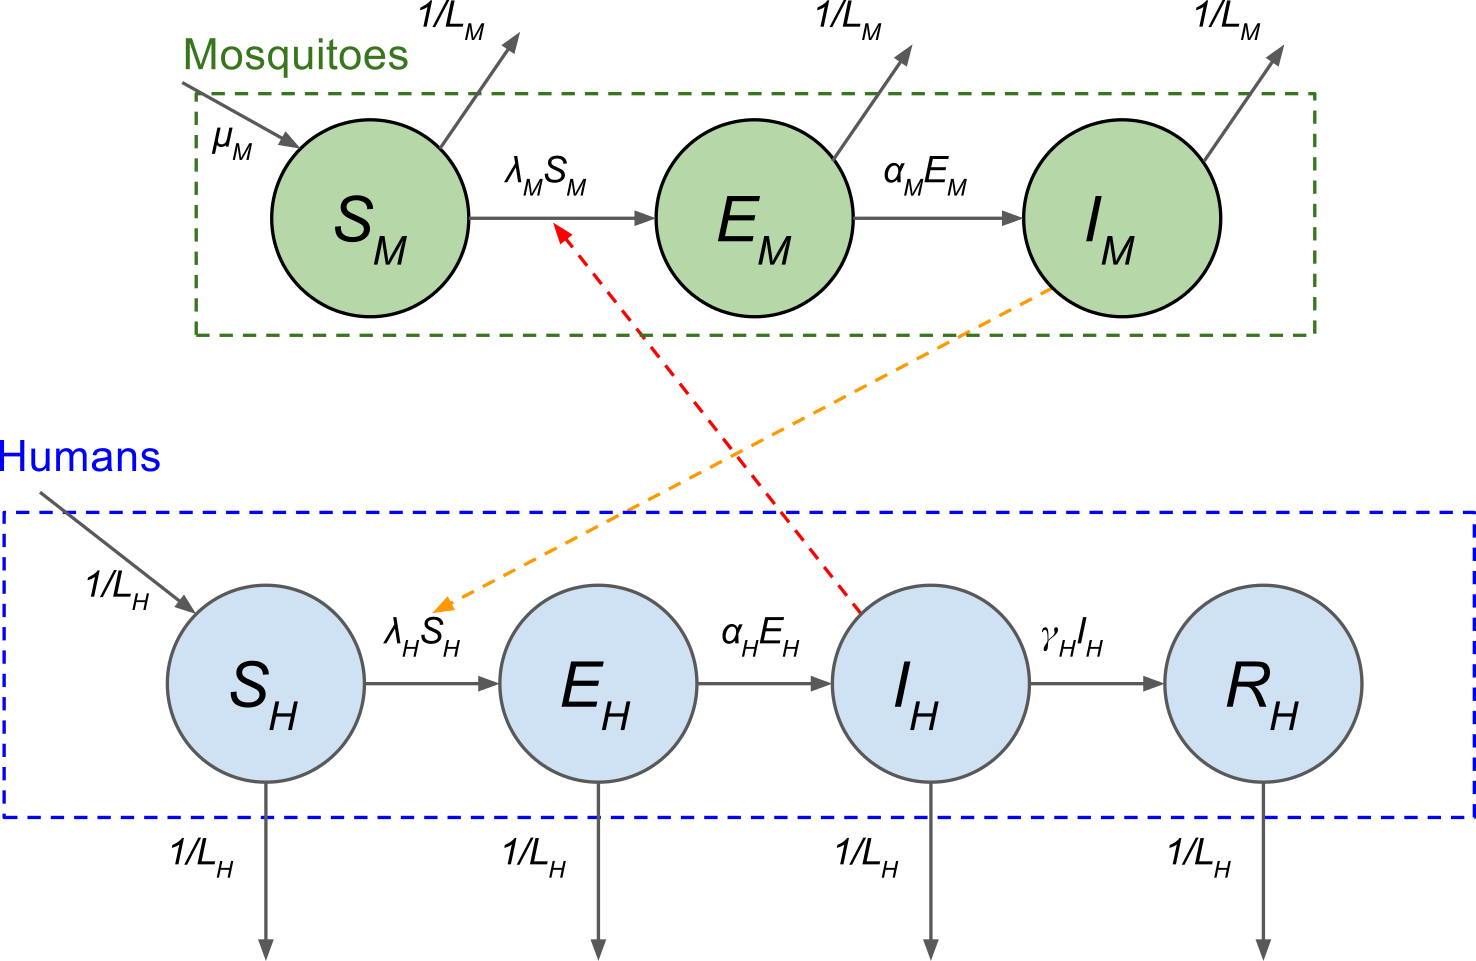
\includegraphics[width=5.20833in]{figures/Fig2.png}
\caption{\textbf{Schematic of forecasting analysis mechanism switch
times.} Left hand column describes the model variant name corresponding
to this mechanism as used in Table S5. The middle column demonstrates
the time at which reporting or behaviour may have switched (green before
the switch, red after). The values shown in the middle column show the
assumed values or contributions of these parameters when the mechanism
is excluded. The Right hand column shows the parameter that is estimated
as a free parameter for that analysis. For example, if microcephaly
reporting is assumed to stay the same, then \(\phi_{m1}=\phi_{m2}=1\)
for all dates. If microcephaly reporting change is the mechanism under
consideration, then \(\phi_{m1}\) is estimated as a free model
parameter. In the joint impact analysis, all parameters in the ``free
parameter'' column are estimated.}
\end{figure}

\section{Fitting to data from Salvador,
Brazil}\label{fitting-to-data-from-salvador-brazil}

We obtained reported acute exanthematous illness (AEI) attributed to
Zika virus and microcephaly incidence in Salvador, Brazil during
2015.{[}23{]} We assumed that reported AEI was proportional to the true
incidence of ZIKV during this time, and scaled the weekly reported
incidence to give a final attack rate in line with seroprevalence
estimates for Salvador. Scaling was done by dividing reported AEI cases
each week by \(\phi_I\) which was calculated as follows:

\begin{equation}
\phi_I = \frac{\sum_t I(t)/N}{AR}
\end{equation}

Where \(I(t)\) is the reported incidence at week \(t\), \(N\) is the
population size of Salvador, and \(AR\) is the reported attack rate
based on seroprevalence. We placed a uniform prior on \(AR\) such that
the total attack rate was between 59.4 and 66.8\%.{[}29{]} \(N\) was
inferred by dividing the total number of reported AEI cases by the
reported total incidence per 1000 persons (giving 2922037); life
expectancy was assumed to be the same as Bahia overall at 73.1 years. We
calculated weekly number of live births by backtracking from the
reported microcephaly incidence in this time period and the total number
of microcephaly cases reported. Paploski et al. report ``367 newborns
with suspected microcephaly (15.6 cases/1,000 newborns during July
2015--February 2016, which peaked at 31.4 cases/1,000 newborns in
December)''``, suggesting that there were 23526 newborns in this period.
We assumed that these births were distributed uniformly across each week
such that there were 420 births per week from July 2015 -- February
2016. The microcephaly reporting rate, \(\phi_m\), was assumed to be
100\%.

Model fitting was then carried out as above; fixing all model parameters
other than \(\phi_I\); \(\alpha\); \(\beta\); and \(c\) as described in
Table S2. Note that in this analysis the SEIR model component is not
included.

\section*{References}\label{references}
\addcontentsline{toc}{section}{References}

\hypertarget{refs}{}
\hypertarget{ref-MacDonald1957}{}
1. MacDonald G. The Epidemiology and Control of Malaria. 1957.

\hypertarget{ref-Diekmann2000}{}
2. Diekmann O, Heesterbeek J. Mathematical Epidemiology of Infectious
Diseases: Model Building, Analysis and Interpretation. John Wiley \&
Sons; 2000.

\hypertarget{ref-Keeling2009}{}
3. Keeling M, Danon L. Mathematical modelling of infectious diseases. Br
Med Bull. 2009;92: 33--42.

\hypertarget{ref-BahiaLifeExpectancy}{}
4. Brazil life expectancy {[}Internet{]}. Available:
\url{ftp://ftp.ibge.gov.br/Tabuas_Completas_de_Mortalidade/Tabuas_Completas_de_Mortalidade_2014/notastecnicas.pdf}

\hypertarget{ref-BahiaPopn}{}
5. Brazil population size {[}Internet{]}. Available:
\url{ftp://ftp.ibge.gov.br/Estimativas_de_Populacao/Estimativas_2015/serie_2001_2015_TCU.pdf}

\hypertarget{ref-ColombiaLifeExpectancy}{}
6. Colombia life expectancy {[}Internet{]}. Available:
\url{https://www.dane.gov.co/files/investigaciones/poblacion/series_proyecciones/proyecc3.xls}

\hypertarget{ref-ColombiaPopn}{}
7. Colombia population size {[}Internet{]}. Available:
\url{http://www.worldometers.info/world-population/colombia-population/}

\hypertarget{ref-Ferguson2016}{}
8. Ferguson NM, Cucunubá ZM, Dorigatti I, Nedjati-Gilani GL, Donnelly
CA, Basáñez M-G, et al. Countering Zika in Latin America. Science.
American Association for the Advancement of Science; 2016;387:
e41918--e41918.
doi:\href{https://doi.org/10.1126/science.aag0219}{10.1126/science.aag0219}

\hypertarget{ref-Johansson2016}{}
9. Johansson MA, Mier-y-Teran-Romero L, Reefhuis J, Gilboa SM, Hills SL.
Zika and the Risk of Microcephaly. N Engl J Med. Massachusetts Medical
Society; 2016;375: 1--4.
doi:\href{https://doi.org/10.1056/NEJMp1605367}{10.1056/NEJMp1605367}

\hypertarget{ref-Zoca2016}{}
10. Microcefalia no Brazil -- 2000 a 2016 {[}Internet{]}. Available:
\url{https://public.tableau.com/profile/bruno.zoca\#!/vizhome/Painel2-microcefalia/Painel2-Microcefalia}

\hypertarget{ref-Faria2016}{}
11. Faria NR, Azevedo R do S da S, Kraemer MUG, Souza R, Cunha MS, Hill
SC, et al. Zika virus in the Americas: Early epidemiological and genetic
findings. Science (80- ). American Association for the Advancement of
Science; 2016;352: 345--349.
doi:\href{https://doi.org/10.1126/science.aaf5036}{10.1126/science.aaf5036}

\hypertarget{ref-deOliveira2017}{}
12. Oliveira WK de, Carmo EH, Henriques CM, Coelho G, Vazquez E,
Cortez-Escalante J, et al. Zika Virus Infection and Associated
Neurologic Disorders in Brazil. N Engl J Med. Massachusetts Medical
Society; 2017;376: 1591--1593.
doi:\href{https://doi.org/10.1056/NEJMc1608612}{10.1056/NEJMc1608612}

\hypertarget{ref-deOliveira2017a}{}
13. Oliveira WK de, França GVA de, Carmo EH, Duncan BB, de Souza
Kuchenbecker R, Schmidt MI. Infection-related microcephaly after the
2015 and 2016 Zika virus outbreaks in Brazil: a surveillance-based
analysis. Lancet. Elsevier; 2017;390: 861--870.
doi:\href{https://doi.org/10.1016/S0140-6736(17)31368-5}{10.1016/S0140-6736(17)31368-5}

\hypertarget{ref-PahoColombia}{}
14. PAHO/WHO. Pan American Health Organization / World Health
Organization. Zika - Epidemiological Report Colombia. September 2017.
Washington, D.C. {[}Internet{]}. 2017. Available:
\url{http://www.paho.org/hq/index.php?option=com_docman\&task=doc_view\&gid=35139\&Itemid=270\&lang=en}

\hypertarget{ref-Cuevas2016b}{}
15. Cuevas EL, Tong VT, Rozo N, Valencia D, Pacheco O, Gilboa SM, et al.
Preliminary Report of Microcephaly Potentially Associated with Zika
Virus Infection During Pregnancy --- Colombia, January--November 2016.
MMWR Morb Mortal Wkly Rep. 2016;65: 1409--1413.
doi:\href{https://doi.org/10.15585/mmwr.mm6549e1}{10.15585/mmwr.mm6549e1}

\hypertarget{ref-ColombiaReport2017}{}
16. 2017 Boletín epidemiológico semana 52 {[}Internet{]}. Available:
\url{https://www.ins.gov.co/buscador-eventos/Paginas/Vista-Boletin-Epidemilogico.aspx}

\hypertarget{ref-BahiaReports}{}
17. Boletim da Microcefalia e outras alterações do SNC sugestivas de
infecção congênita. Bahia, 2016 {[}in Portuguese{]} {[}Internet{]}.
Available:
\url{http://www.saude.ba.gov.br/wp-content/uploads/2017/11/2017-Boletim-epidemiol\%C3\%B3gico-da-Microcefalia-n.-01.pdf}

\hypertarget{ref-BahiaReportsB}{}
18. Situação Epidemiológica das Arboviroses. Bahia, 2016 {[}in
Portuguese{]} {[}Internet{]}. Available:
\url{http://www.saude.ba.gov.br/wp-content/uploads/2017/11/Boletim-epidemiológico-20-arboviroses-31-dezembro-2016.pdf}

\hypertarget{ref-RioReports}{}
19. Boletim Epidemiológico Dez/2016 SE 52 {[}in Portuguese{]}
{[}Internet{]}. Available:
\url{http://www.saude.rn.gov.br/Conteudo.asp?TRAN=ITEM\&TARG=110749\&ACT=\&PAGE=0\&PARM=\&LBL=Arboviroses}

\hypertarget{ref-RioReportsB}{}
20. Atualização da Situação Epidemiológica da Microcefalia e/ou outras
alterações do sistema nervoso central de causas infecciosas no Rio
Grande do Norte {[}in Portuguese{]} {[}Internet{]}. Available:
\url{http://adcon.rn.gov.br/ACERVO/sesap/DOC/DOC000000000140265.PDF}

\hypertarget{ref-PernambucoReports}{}
21. PAHO/WHO. Pan American Health Organization / World Health
Organization. Zika Epidemiological Update, 26 May 2016. Washington, D.C.
{[}Internet{]}. 2016. Available:
\url{https://www.paho.org/hq/index.php?option=com_docman\&task=doc_view\&Itemid=270\&gid=34797\&lang=en}

\hypertarget{ref-PahoPernambuco}{}
22. PAHO/WHO. Pan American Health Organization / World Health
Organization. Zika Epidemiological Update, 26 May 2016. Washington, D.C.
2016. Available:
\url{https://www.paho.org/hq/dmdocuments/2016/2016-may-26-cha-epi-update-zika-virus.pdf}

\hypertarget{ref-Paploski}{}
23. Paploski IA, Prates APP, Cardoso CW, Kikuti M, Silva MMO, Waller LA,
et al. Time Lags between Exanthematous Illness Attributed to Zika Virus,
Guillain-Barré Syndrome, and Microcephaly, Salvador, Brazil. Emerg
Infect Dis. 2016;22: 1438--1444.
doi:\href{https://doi.org/10.3201/eid2208.160496}{10.3201/eid2208.160496}

\hypertarget{ref-Sheppard1969}{}
24. Sheppard PM, Macdonald WW, Tonn RJ, Grab B. The Dynamics of an Adult
Population of Aedes aegypti in Relation to Dengue Haemorrhagic Fever in
Bangkok. J Anim Ecol. British Ecological Society; 1969;38: 661.
doi:\href{https://doi.org/10.2307/3042}{10.2307/3042}

\hypertarget{ref-Lessler2016}{}
25. Lessler J, Ott CT, Carcelen AC, Konikoff JM, Williamson J, Bi Q, et
al. Times to key events in Zika virus infection and implications for
blood donation: a systematic review. Bull World Health Organ. World
Health Organization; 2016;94: 841--849.
doi:\href{https://doi.org/10.2471/BLT.16.174540}{10.2471/BLT.16.174540}

\hypertarget{ref-Majumder2016a}{}
26. Majumder MS, Cohn E, Fish D, Brownstein JS. Estimating a feasible
serial interval range for Zika fever. Bull World Heal Organ. 2016;
doi:\href{https://doi.org/10.2471/BLT.16.171009}{10.2471/BLT.16.171009}

\hypertarget{ref-ReportingChange}{}
27. Epidemiological Alert. Zika virus infection 7 May 2015
{[}Internet{]}. Available:
\url{http://www.paho.org/hq/index.php?option=com_docman\&task=doc_view\&Itemid=270\&gid=30075}

\hypertarget{ref-ProtocolCZS}{}
28. Protocol for surveillance and response to the occurrence of
microcephaly and/or central nervous system (CNS) alterations {[}in
Portuguese{]} {[}Internet{]}. Available:
\url{http://portalarquivos.saude.gov.br/images/pdf/2016/marco/24/Microcefalia-Protocolo-vigil--ncia-resposta-versao2.1.pdf}

\hypertarget{ref-Netto}{}
29. Netto EM, Moreira-Soto A, Pedroso C, Höser C, Funk S, Kucharski AJ,
et al. High Zika Virus Seroprevalence in Salvador, Northeastern Brazil
Limits the Potential for Further Outbreaks. MBio. American Society for
Microbiology; 2017;8: e01390--17.
doi:\href{https://doi.org/10.1128/mBio.01390-17}{10.1128/mBio.01390-17}

\nolinenumbers


\end{document}

